%%%%%%%%%%%%%%%%%%%%%%%%%%%%%%%%%%%%%%%%%%%%%%%%%%%%%%%%%%%%%%%%%%%%%%%%%%%%%%%%
%% Plantilla de memoria en LaTeX para la ETSIT - Universidad Rey Juan Carlos
%%
%% Por Gregorio Robles <grex arroba gsyc.urjc.es>
%%     Grupo de Sistemas y Comunicaciones
%%     Escuela Técnica Superior de Ingenieros de Telecomunicación
%%     Universidad Rey Juan Carlos
%% (muchas ideas tomadas de Internet, colegas del GSyC, antiguos alumnos...
%%  etc. Muchas gracias a todos)
%%
%% La última versión de esta plantilla está siempre disponible en:
%%     https://github.com/gregoriorobles/plantilla-memoria
%%
%% Para obtener PDF, ejecuta en la shell:
%%   make
%% (las imágenes deben ir en PNG o JPG)

%%%%%%%%%%%%%%%%%%%%%%%%%%%%%%%%%%%%%%%%%%%%%%%%%%%%%%%%%%%%%%%%%%%%%%%%%%%%%%%%

\documentclass[a4paper, 12pt]{book}
%\usepackage[T1]{fontenc}

\usepackage[a4paper, left=2.5cm, right=2.5cm, top=3cm, bottom=3cm]{geometry}
\usepackage{times}
\usepackage[utf8]{inputenc}
\usepackage[spanish]{babel} % Comenta esta línea si tu memoria es en inglés
\usepackage{url}
%\usepackage[dvipdfm]{graphicx}
\usepackage{graphicx}
\usepackage{float}  %% H para posicionar figuras
\usepackage[nottoc, notlot, notlof, notindex]{tocbibind} %% Opciones de índice
\usepackage{latexsym}  %% Logo LaTeX
\usepackage[dvipsnames]{xcolor} %%Color de palabras
\usepackage{xcolor}

\newif\ifdraft
\drafttrue
%\draftfalse
\input{macros}


\title{Memoria del Proyecto}
\author{Nombre del autor}

\renewcommand{\baselinestretch}{1.5}  %% Interlineado

\begin{document}

\renewcommand{\refname}{Bibliografía}  %% Renombrando
\renewcommand{\appendixname}{Apéndice}

%%%%%%%%%%%%%%%%%%%%%%%%%%%%%%%%%%%%%%%%%%%%%%%%%%%%%%%%%%%%%%%%%%%%%%%%%%%%%%%%
% PORTADA

\begin{titlepage}
\begin{center}
\includegraphics[scale=0.8]{img/URJ_logo_Color_POS.png}

\vspace{1.75cm}

\Large
GRADO EN INGENIERÍA EN SISTEMAS AUDIOVISUALES Y MULTIMEDIA

\vspace{0.4cm}

\large
Curso Académico 2020/2021

\vspace{0.8cm}

Trabajo Fin de Grado

\vspace{2.5cm}

\LARGE
IMPLEMENTACIÓN DE FUNCIONALIDADES EN LEARNINGML

\vspace{4cm}

\large
Autor : Isaac Merchán Blanco\\
Tutor : Dr. Gregorio Robles\\
Co-tutor: Juan David Rodríguez García
\end{center}
\end{titlepage}

\newpage
\mbox{}
\thispagestyle{empty} % para que no se numere esta pagina


%%%%%%%%%%%%%%%%%%%%%%%%%%%%%%%%%%%%%%%%%%%%%%%%%%%%%%%%%%%%%%%%%%%%%%%%%%%%%%%%
%%%% Para firmar
\clearpage
\pagenumbering{gobble}
\chapter*{}

\vspace{-4cm}
\begin{center}
\LARGE
\textbf{Trabajo Fin de Grado}

\vspace{1cm}
\large
IMPLEMENTACIÓN DE FUNCIONALIDADES EN LEARNINGML

\vspace{1cm}
\large
\textbf{Autor :} Isaac Merchán Blanco \\
\textbf{Tutor :} Dr. Gregorio Robles \\
\textbf{Co-tutor :} Juan David Rodríguez García

\end{center}

\vspace{1cm}
La defensa del presente Proyecto Fin de Carrera se realizó el día \qquad$\;\,$ de \qquad\qquad\qquad\qquad \newline de 2021, siendo calificada por el siguiente tribunal:


\vspace{0.5cm}
\textbf{Presidente:}

\vspace{1.2cm}
\textbf{Secretario:}

\vspace{1.2cm}
\textbf{Vocal:}


\vspace{1.2cm}
y habiendo obtenido la siguiente calificación:

\vspace{1cm}
\textbf{Calificación:}


\vspace{1cm}
\begin{flushright}
Fuenlabrada, a \qquad$\;\,$ de \qquad\qquad\qquad\qquad de 2021
\end{flushright}

%%%%%%%%%%%%%%%%%%%%%%%%%%%%%%%%%%%%%%%%%%%%%%%%%%%%%%%%%%%%%%%%%%%%%%%%%%%%%%%%
%%%% Dedicatoria

\chapter*{}
\pagenumbering{Roman} % para comenzar la numeracion de paginas en numeros romanos
\begin{flushright}
\textit{Dedicado a \\
mi familia y amigos}
\end{flushright}

%%%%%%%%%%%%%%%%%%%%%%%%%%%%%%%%%%%%%%%%%%%%%%%%%%%%%%%%%%%%%%%%%%%%%%%%%%%%%%%%
%%%% Agradecimientos

\chapter*{Agradecimientos}
%\addcontentsline{toc}{chapter}{Agradecimientos} % si queremos que aparezca en el índice
\markboth{AGRADECIMIENTOS}{AGRADECIMIENTOS} % encabezado 

Quiero agradecer a mis padres quienes han sido capaces de aguantar mis peores momentos durante esta carrera. A mi madre que desde pequeño siempre ha estado ayudándome con todo lo que he necesitado y confiando en mi. Y a mi padre que aunque no pase tanto tiempo con él me ha inculcado unos valores y una forma de ver la vida que me han llevado a ser quien soy a día de hoy.

Quería agradecer también a mis amigos por estar siempre dispuestos a sacar un rato para vernos y hablar, esos momentos de descanso también forman parte de esto y sin ellos nada sería lo mismo.

Gracias también a mis compañeros con los que he pasado estos últimos años de mi vida y una etapa muy importante, sin ellos esto hubiera sido aún más difícil. Han hecho que las clases, las tardes de estudio, las prácticas y en general la carrera, sea más divertida.

Por último, agradecer a Gregorio su manera de explicar y su disposición para ayudarme siempre que he necesitado algo y a Juanda por dejarme colaborar en su página.


%%%%%%%%%%%%%%%%%%%%%%%%%%%%%%%%%%%%%%%%%%%%%%%%%%%%%%%%%%%%%%%%%%%%%%%%%%%%%%%%
%%%% Resumen

\chapter*{Resumen}
%\addcontentsline{toc}{chapter}{Resumen} % si queremos que aparezca en el índice
\markboth{RESUMEN}{RESUMEN} % encabezado

El \emph{machine learning} (aprendizaje automático) es algo que está a la orden del día, se usa para prácticamente todo, desde coches que se conducen solos, hasta recomendaciones de series o películas en cualquier plataforma. \texttt{LearningML} pretende acercar esta tecnología a cualquier persona que sin grandes conocimientos sobre el tema pueda probar y ver como la web, primero aprende y después clasifica una imagen o un texto utilizando el algoritmo que elija el usuario.
 
Este proyecto consiste en implementar dos nuevos algoritmos de \emph{machine learning} para la aplicación web  \texttt{LearningML}\footnote{\url{https://learningml.org/editor/}}. Por un lado el algoritmo de K-NN o K-vecinos más cercanos y por otro el de Naive Bayes. Para ello ha sido necesario cambiar la estructura de la aplicación web de manera que de cara a futuras actualizaciones o mejoras se puedan hacer de manera más sencilla.

\texttt{LearningML} usa el lenguaje TypeScript y está creada con Angular, por lo que después de la reestructuración solo ha sido necesario crear dos nuevos servicios, uno para cada clasificador, y llamar a sus funciones desde otro servicio que está por encima de ambos y elige que modelo usar. Dentro de estos servicios, se han construido dos funciones: una para entrenar el modelo y otra para probarlo. Estas funciones se lanzan de manera asíncrona para que encaje con lo que ya estaba construido previamente.




%%%%%%%%%%%%%%%%%%%%%%%%%%%%%%%%%%%%%%%%%%%%%%%%%%%%%%%%%%%%%%%%%%%%%%%%%%%%%%%%
%%%% Resumen en inglés

\chapter*{Summary}
%\addcontentsline{toc}{chapter}{Summary} % si queremos que aparezca en el índice
\markboth{SUMMARY}{SUMMARY} % encabezado

Machine learning is something that is the order of the day, it is used for practically everything, from self-driving cars to recommendations of series or films on any platform. \texttt{LearningML} aims to bring this technology to anyone without great knowledge on the subject can try and see how the web, first learns and then classifies an image or text using the algorithm of the user's choice.

This project consists of implementing two new algorithms of machine learning on the existing LearningML web application. On the one hand, the K-NN or K-nearest neighbours algorithm and on the other hand, the Naive Bayes algorithm. To do this, it has also been necessary to change the structure of the website so that future updates or improvements can be made more easily.

This web application uses the TypeScript language and is created with Angular, so after the restructuring it has only been necessary to create two new services, one for each classifier, and call their functions from another service that is above both and chooses which model to use. Within these services, two functions have been built, one to train the model and one to test it. These functions are launched asynchronously to fit in with what was previously built.




%%%%%%%%%%%%%%%%%%%%%%%%%%%%%%%%%%%%%%%%%%%%%%%%%%%%%%%%%%%%%%%%%%%%%%%%%%%%%%%%
%%%%%%%%%%%%%%%%%%%%%%%%%%%%%%%%%%%%%%%%%%%%%%%%%%%%%%%%%%%%%%%%%%%%%%%%%%%%%%%%
% ÍNDICES %
%%%%%%%%%%%%%%%%%%%%%%%%%%%%%%%%%%%%%%%%%%%%%%%%%%%%%%%%%%%%%%%%%%%%%%%%%%%%%%%%

% Las buenas noticias es que los índices se generan automáticamente.
% Lo único que tienes que hacer es elegir cuáles quieren que se generen,
% y comentar/descomentar esa instrucción de LaTeX.

%%%% Índice de contenidos
\tableofcontents 
%%%% Índice de figuras
\cleardoublepage
%\addcontentsline{toc}{chapter}{Lista de figuras} % para que aparezca en el indice de contenidos
\listoffigures % indice de figuras
%%%% Índice de tablas
%\cleardoublepage
%\addcontentsline{toc}{chapter}{Lista de tablas} % para que aparezca en el indice de contenidos
%\listoftables % indice de tablas


%%%%%%%%%%%%%%%%%%%%%%%%%%%%%%%%%%%%%%%%%%%%%%%%%%%%%%%%%%%%%%%%%%%%%%%%%%%%%%%%
%%%%%%%%%%%%%%%%%%%%%%%%%%%%%%%%%%%%%%%%%%%%%%%%%%%%%%%%%%%%%%%%%%%%%%%%%%%%%%%%
% INTRODUCCIÓN %
%%%%%%%%%%%%%%%%%%%%%%%%%%%%%%%%%%%%%%%%%%%%%%%%%%%%%%%%%%%%%%%%%%%%%%%%%%%%%%%%

\cleardoublepage
\chapter{Introducción}
\label{sec:intro} % etiqueta para poder referenciar luego en el texto con~\ref{sec:intro}
\pagenumbering{arabic} % para empezar la numeración de página con números

Hoy en día vivimos en un mundo digital en el que hay una cantidad inmensa de datos. La obtención de estos crece a un ritmo exponencial: solo en 2018 se generaron 33 zettabytes (un zettabyte equivale a 1.000 millones de terabytes), lo que equivale a 16,5 veces más que en 2009~\cite{webstatista}. A pesar de esto, solo somos capaces de procesar el 0,5\%~\cite{machinelearning} y ese porcentaje cada vez va a menos ya que no se incrementa de la misma forma la capacidad de obtención que de procesado. El principal problema de esta cuestión se debe a la complejidad y cantidad de los datos, pues los humanos no somos capaces muchas veces de extraer información útil de esos datos. Esto ha hecho que se fomente el estudio de distintos campos, uno de ellos es el \emph{machine learning}. Estas limitaciones mencionadas anteriormente desaparecen en el momento en el que el \emph{machine learning} entra en juego, ya que es capaz de procesar grandes cantidades de datos complejos y transformarlos en información legible y fácil de analizar por los los humanos.

El \emph{machine learning} (o aprendizaje automático) es la rama de la inteligencia artificial que trata de implementar el aprendizaje automático de máquinas a través de un entrenamiento. A pesar de ser un concepto relativamente nuevo, se basa en campos de estudio anteriores como la modelación estadística y o el reconocimiento de patrones.

\section{Presentación de la aplicación}
\label{sec:presentacionaplicacion}

Este Trabajo Fin de Grado tiene como principal objetivo la integración de los algoritmos de aprendizaje automático de Naive Bayes y K-NN en la web de LearningML que actualmente solo utiliza el método de redes neuronales para clasificar imágenes o texto.

\texttt{LearningML} es una aplicación web creada por Juan David Rodríguez García utilizando Angular y esta construida de tal manera que cualquier persona sin grandes conocimientos sobre el aprendizaje automático pueda crear un modelo, entrenarlo y después probarlo.

La aplicación web además permite descargar el modelo creado en un archivo JSON para después poder cargarlo sin necesidad de crearlo de nuevo, esto es muy útil ya que de esta manera no se tienen que volver a introducir todas las entradas para el aprendizaje, sino que directamente se puede importar un modelo creado previamente e introducir una entrada para ver su funcionamiento.

También tiene la opción de registrarse y poder guardar los modelos en tu cuenta o incluso tener proyectos compartidos entre varias personas. Por último, permite crear un modelo en Scratch y utilizarlo en la web, aunque esta parte no se verá durante este trabajo.


\section{Estructura de la memoria}
\label{sec:estructura}

La memoria empieza con un resumen, en el que se explica brevemente en que consiste el proyecto, así como las tecnologías que se han usado para llevarlo a cabo. A continuación, se sitúan los agradecimiento y los índices, tanto el general como el de figuras. Finalmente, van los seis capítulos en los que se divide la memoria.

\begin{itemize}
  \item \textbf{Capítulo 1: Introducción.} En el primer capítulo se hace una breve explicación de en que consiste la web de LearningML y la estructura que va a seguir el trabajo.
  
  \item \textbf{Capítulo 2: Objetivos.} En este capítulo se describen los objetivos principales y específicos del trabajo y la planificación temporal de este.
  
  \item \textbf{Capítulo 3: Estado del arte.} Se trata de una breve explicación sobre la mayoría de las tecnologías utilizadas en el desarrollo de la aplicación web.

  \item \textbf{Capítulo 4: Diseño e implementación.} Se describe de manera detallada tanto los cambios previos en la estructura como la arquitectura final de la aplicación web así como la implementación de los dos modelos de aprendizaje.
  
  \item \textbf{Capítulo 5: Experimentos y validación.} Se comprueba si funcionan correctamente las funcionalidades implementadas en la web de LearningML.
  
  \item \textbf{Capítulo 6: Conclusiones.} Por último, se repasa todo lo aprendido durante el desarrollo del proyecto y se comentan algunas mejoras o funciones que se podrían implementar en un futuro.
  
\end{itemize}



%%%%%%%%%%%%%%%%%%%%%%%%%%%%%%%%%%%%%%%%%%%%%%%%%%%%%%%%%%%%%%%%%%%%%%%%%%%%%%%%
%%%%%%%%%%%%%%%%%%%%%%%%%%%%%%%%%%%%%%%%%%%%%%%%%%%%%%%%%%%%%%%%%%%%%%%%%%%%%%%%
% OBJETIVOS %
%%%%%%%%%%%%%%%%%%%%%%%%%%%%%%%%%%%%%%%%%%%%%%%%%%%%%%%%%%%%%%%%%%%%%%%%%%%%%%%%

\cleardoublepage % empezamos en página impar
\chapter{Objetivos} % título del capítulo (se muestra)
\label{chap:objetivos} % identificador del capítulo (no se muestra, es para poder referenciarlo)

\section{Objetivo general} % título de sección (se muestra)
\label{sec:objetivo-general} % identificador de sección (no se muestra, es para poder referenciarla)

Este Trabajo Fin de Grado consiste en añadir a la aplicación web de LearningML los algoritmos de aprendizaje automático de Bayes y K-NN de manera intuitiva e independientemente de si se quieren clasificar textos o imágenes.

\section{Objetivos específicos}
\label{sec:objetivos-especificos}

Para la realización del objetivo general se han planteado los siguientes objetivos específicos:
\begin{itemize}
  
	\item Reorganizar la manera de trabajar de LearningML para separar la obtención de datos del algoritmo utilizado.
 
	\item Implementar el algoritmo de Bayes y K-NN para que funcionen como dos clasificadores de tal forma que primero entrenen con las entradas de aprendizaje y luego evalúen otra entrada proporcionada por el usuario y la asigne correctamente a uno de los grupos creados previamente.
  
	\item Añadir en la interfaz una manera de poder elegir el tipo de algoritmo que se quiere utilizar de forma independiente a si los elementos a clasificar son texto o imágenes.

	\item Dejar que el usuario pueda tocar algunos de los parámetros de los clasificadores.

\end{itemize}


\section{Planificación temporal}
\label{sec:planificacion-temporal}

La primera idea que tuve de empezar con el Trabajo Fin de Grado (TFG) fue en enero de 2021 y quería hacerlo a la vez que las prácticas entonces me puse en contacto con Gregorio y me comentó esto. Me llamo la atención la aplicación web de LearningML, ya que recuerdo haber utilizado Scratch en el colegio y me parecía interesante aportar algo aunque sea de manera indirecta a que los niños se interesen por la programación.

En principio este proyecto iba a ser tanto prácticas como TFG y le iba a poder dedicar bastante horas todos los días, sin embargo, me aceptaron en unas prácticas y no tuve tanto tiempo ya que estas eran de jornada completa. Además de esto, aun tenía una asignatura pendiente así que era difícil establecer un horario concreto para dedicarle tiempo al proyecto. Cuando no tenía un examen cerca, al salir de trabajar me ponía con ello un rato y luego los fines de semana por la mañana también le dedicaba algo de tiempo.

Recuerdo que primero tuve que aprender cómo funcionaba Angular y TypeScript con un curso que tiene Juanda. Estuve practicando y familiarizándome con la forma de trabajar en Angular.

Después tuve varias reuniones con Juanda (creador de LearningML) para ver cómo funcionaba la aplicación de LearningML y donde había que añadir los cambios.
También tuve que buscar que bibliotecas ya construidas de Bayes y K-NN que pudiéramos adaptar para usarlas en la aplicación web y finalmente ponerme a ello. Para K-NN si que conseguí encontrar una biblioteca que me sirvió aunque por cómo se obtienen los datos, había que procesarlos de nuevo antes de usarlos. Para Bayes no encontré nada y tuve que crear el clasificador desde cero lo que me llevo algo más de tiempo que en el otro caso.
Por último, quedaba la tarea de trasladar todo eso al papel. Me puse en contacto con mi tutor y enseguida me paso una plantilla con los apartados a rellenar y comencé a hacerlo hasta que finalmente, con no mucho tiempo de margen para entregar el trabajo, terminé.


%%%%%%%%%%%%%%%%%%%%%%%%%%%%%%%%%%%%%%%%%%%%%%%%%%%%%%%%%%%%%%%%%%%%%%%%%%%%%%%%
%%%%%%%%%%%%%%%%%%%%%%%%%%%%%%%%%%%%%%%%%%%%%%%%%%%%%%%%%%%%%%%%%%%%%%%%%%%%%%%%
% ESTADO DEL ARTE %
%%%%%%%%%%%%%%%%%%%%%%%%%%%%%%%%%%%%%%%%%%%%%%%%%%%%%%%%%%%%%%%%%%%%%%%%%%%%%%%%

\cleardoublepage
\chapter{Estado del arte}
\label{chap:estado}

En este apartado veremos tanto las tecnologías utilizadas como una breve explicación sobre lo que es el modelo de Bayes y de K-NN.

\section{HTML5} 
\label{sec:html5}

HTML~\cite{htmlw3,htmlwhat} (HyperText Markup Language) es un lenguaje de marcado que se utiliza para describir la estructura de las páginas web. HTML5 es la quinta versión de este lenguaje. A lo largo de todas las versiones se han incorporado y eliminado diferentes características, con el fin de hacerlo más eficiente y facilitar el desarrollo web compatible con distintos navegadores y plataformas, y manteniéndose también la retro compatibilidad con las versiones anteriores.
A pesar de ser un estándar a cargo del Consorcio WWW, fue la asociación WHATWG, formada por Apple, Opera y Mozilla, la que publicó el primer borrador de HTML5 cuando W3C decidió dejar de evolucionar HTML. Más tarde W3C y WHATWG trabajaron juntos durante varios años en el desarrollo de HTML5, hasta que se separaron debido a sus diferentes objetivos, W3C quería publicar una versión terminada mientras que WHATWG quería seguir trabajando, manteniendo HTML5 en constante evolución.
Algunas de las principales características de HTML5 son:
\begin{itemize}
	\item Incorpora nuevas etiquetas que especifican la semántica del contenido, ayudando a interpretar mejor la página. Antes solo teníamos \textless{}div\textgreater{} para definir cualquier sección, ahora podemos utilizar \textless{}header\textgreater{}, \textless{}nav\textgreater{}, \textless{}section\textgreater{}, \textless{}footer\textgreater{}, entre otros.

	\item Ofrece también mejoras en los formularios como validaciones, nuevos tipos de campos (email, date, range, etc) y nuevos atributos, por ejemplo, multiple, placeholder o form.

	\item Cuenta con numerosas APIs. Algunas de ellas son:

	\begin{itemize}

		\item Audio y vídeo: permite incrustar elementos de audio y vídeo y reproducirlo desde el propio navegador.

		\item Web Storage: permite almacenar datos del lado del cliente, cuando la sesión está activa.

        	\item Canvas: que permite hacer dibujos, juegos, animaciones, etc.

		\item Geolocalización: permite mostrar e interactuar con un mapa de Google Maps.

	\end{itemize}
\end{itemize}

\section{TypeScript} 
\label{sec:typescript}

TypeScript~\cite{typescript} es un lenguaje de programación, de código abierto y desarrollado por Microsoft.
Nació como una necesidad de mejorar algunos problemas de JavaScript, entre ellos el hecho de que es bastante complicado crear aplicaciones a gran escala con JavaScript. Está pensado para el desarrollo de aplicaciones robustas y escalables, y se puede utilizar tanto en el lado del cliente como en el servidor junto a Node.js.

TypeScript es un superconjunto de JavaScript, es decir, se trata de un lenguaje creador a partir de JavaScript. Los programas de JavaScript son programas válidos de TypeScript. Esto permite integrar TypeScript en proyectos ya existentes, sin tener que rehacer todo el proyecto en TypeScript, ya que todo el código TypeScript se puede compilar en JavaScript nativo.
Las características más importantes de TypeScript son:

\begin{itemize}

	\item Tenemos a nuestra disposición las herramientas de JavaScript ES6 (Ecmascript 6). De esta forma se mantiene actualizado con las últimas mejoras de JavaScript.

	\item Cuenta con un tipado estático, por tanto, al crear variables podemos añadir el tipo de dato, así podemos evitar errores en tiempo de ejecución.

	\item Objetos basados en clases, lo que hace más sencilla la programación orientada a objetos y añade más funcionalidad.

\end{itemize}

\section{Node.js} 
\label{sec:nodejs}

Node~\cite{nodejs} es un entorno de ejecución de JavaScript controlado por eventos asíncronos, diseñado para construir aplicaciones de red escalables.
Fue creado por Ryan Dahl en 2009 y está influenciado por algunos sistemas como Event Machine de Ruby o Twisted de Python.

Cuando se utiliza JavaScript en el lado del cliente, es el navegador quien, a través de un programa interno (un motor), interpreta el código JavaScript. De este mismo modo, Node.js proporciona un entorno de ejecución JavaScript del lado del servidor, haciendo uso del motor V8 de Google, que se encarga de interpretar el código y ejecutarlo.
El motor V8 es el que Google usa en su navegador Chrome y es posible descargarlo e introducirlo en cualquier aplicación.

Node.js está pensado para soportar grandes cantidades de solicitudes muy altas gracias a su naturaleza asíncrona. El modelo de concurrencia más común está basado en la utilización de hilos del sistema operativo. Se genera un nuevo hilo para cada conexión, de modo que a mayor cantidad de personas, mayor cantidad de recursos consumidos del servidor y mayor número de servidores son necesarios. Node.js emplea un único hilo y un bucle de eventos asíncrono. Las nuevas peticiones son tratadas como eventos en este bucle, de esta forma, no se produce ningún tipo de bloqueo en el flujo de trabajo.

\section{Archivos JSON} 
\label{sec:archivosjson}

JSON (JavaScript Object Notation - Notación de Objetos de JavaScript) es un formato de intercambio de datos~\cite{json}. Es sencillo tanto de escribir como de leer, lo que facilita que tanto los humanos como las máquinas sean capaces de utilizarlos y generarlos. Aunque esta basado en un subconjunto del lenguaje de programación JavaScript, es un formato de texto completamente independiente del lenguaje.

En el siguiente texto en formato JSON podemos ver las dos estructuras que nos ofrece, una colección de pares nombre/valor y una lista de valores. En el ejemplo, vemos que el tipo de clasificador será de texto en este caso y que dentro de los datos tendremos dos etiquetas, una de vocales con una lista de las entradas que pertenecen a esta etiqueta y otra de consonantes. 

\begin{verbatim}
{
    "type": "text",
    "data": {
        "vocales": [
            "aaa",
            "eee",
            "iii"
        ],
        "consonantes": [
            "sss",
            "ddd",
            "fff"
        ]
    }
}
\end{verbatim}


\section{Angular} 
\label{sec:angular}

Angular~\cite{angular} es un \emph{framework} de código abierto diseñado por Google. Permite crear aplicaciones web de una sola página, lo que se denomina SPA (Single Page Application). Utiliza TypeScript y HTML para el desarrollo de las aplicaciones web. 

Angular permite separar el \emph{frontend} del \emph{backend} y sigue un modelo MVC (Modelo-Vista-Controlador), que se verá cómo funciona en el siguiente apartado. De esta forma, las modificaciones y las actualizaciones de las aplicaciones son rápidas y sencillas. 

Una de las principales ventajas de este \emph{framework} y de las páginas SPA es la velocidad de carga entre las diferentes vistas de la aplicación. Cuando se cambia de vista no se recarga la página si no que éstas se cargan de manera dinámica, rápida y reactiva. 

Angular dispone de varias versiones y en cada una de ellas se han ido implementando mejoras en dicho \emph{framework}. La primera versión de Angular, se conoce como AngularJS, y es la más distinta a las demás. El resto son actualizaciones de Angular 2. Cuando se definió la segunda versión se decidió modificar el nombre del \emph{framework} y dejarlo como Angular. La última versión es la 12, liberada en mayo de este año.

La arquitectura de una aplicación Angular se basa en clases de cuatro tipos distintos (módulos, componentes, servicios y directivas). Estas clases se identifican a través de decoradores, que permiten cargar los metadatos necesarios que determinan a Angular como debe usar dichas clases.

\textbf{Módulos}.

Los módulos suministran el contexto de compilación de los componentes, es decir, es aquí donde se definen los diferentes componentes que van a formar la aplicación, las dependencias, las clases que actúan como servicios en la aplicación y las rutas de navegación que establecen las vistas de la aplicación. 

Toda aplicación angular tiene un módulo principal o raíz. Este módulo suele recibir el nombre de \emph{AppModule} y es el que inicia el sistema de arranque de la aplicación.

Al igual que en JavaScript, los módulos de Angular permiten importar y exportar funcionalidades proporcionadas por otros módulos, por lo que una aplicación puede tener más de un módulo, siendo cada uno de ellos independiente. La manera en que se organizan estos módulos ayuda a la creación de aplicaciones más complejas y a la reutilización de código. Además, permite que la carga inicial sea mínima, ya que cada módulo se carga a petición, es decir, cuando se va a utilizar. 

\textbf{Componentes}. 

Las aplicaciones Angular tienen un componente que es el nexo de unión entre los diferentes componentes que forman la aplicación y el modelo de objeto del documento de la página (DOM). Los componentes son los que tienen la lógica y los datos de la aplicación. Son los que controlan las diferentes plantillas HTML que se cargan cuando se modifican las URLs. Estas plantillas HTML son las vistas que forman la interfaz de usuario.

De la misma forma que las aplicaciones diseñadas con Angular pueden tener más de un módulo, también pueden tener subcomponentes, que se pueden relacionar entre sí mediante dos tipos de vinculación de datos, eventos y propiedades. A través de los eventos, la aplicación responde a las entradas del usuario actualizando los datos. A través de las propiedades, se envían valores calculados de los datos de la aplicación a los HTMLs que forman las vistas. Esta vinculación de datos se puede producir en ambas direcciones, es decir, igual que los datos de la aplicación pueden modificar los HTMLs, los cambios en el DOM pueden modificar los datos de la aplicación.

El decorador @Component es el que determina que una clase actúe como un componente. 

\textbf{Servicios}

Los servicios son clases en las que se definen datos o funcionalidades generales que no están asociadas a una determinada vista. Son usados para compartir datos y operaciones entre componentes. También es donde se suele realizar toda la operativa de las peticiones a la API de las aplicaciones. Deben llevar el decorador @Injectable, pues es el que permite obtener los metadatos necesarios para que otras clases puedan inyectar sus dependencias. 

\textbf{Directivas}

Las directivas son clases en las que se definen los términos claves que se usan en las plantillas. Cuando se carga una vista, Angular procesa estos términos clave que modifican el HTML y el DOM de la aplicación. Por tanto, una plantilla, además de utilizar HTML para definir la vista, usa marcas propias de Angular que son estas directivas. 

Existen dos clases de directivas: las de atributo, que modifican el comportamiento del componente, y las estructurales, que únicamente modifican la apariencia. 

Angular dispone de un enrutador, módulo que contiene un servicio para definir las rutas de navegación de la aplicación. Este módulo se ajusta a las convenciones de los navegadores. Es decir, tanto si se pone la URL en la barra de direcciones, como si se pincha un enlace en la aplicación, como si se hace \emph{click} en el botón de retroceso o avance, se carga a la página correspondiente. El enrutador es el que muestra u oculta una vista. Cada vez que se modifica la URL, el enrutador se encarga de añadir la ruta en el historial del navegador, es esto lo que permite que los botones de retroceso y avance funcionen. Cada ruta de navegación está asociado a un componente. 

\subsection{MVC} 
\label{sec:mvc}

Las aplicaciones web se suelen desarrollar siguiendo una serie de pautas. El patrón que sigue Angular es el Modelo Vista Controlador (MVC), cuyos elementos son~\cite{mvc} :

\begin{itemize}
  
	\item \textbf{Modelo:} es la representación de los datos de toda la aplicación y, por tanto, maneja las consultas y todas las acciones relacionadas con base de datos en caso de que las hubiera. También tratará los datos para cumplir con las funcionalidades de la aplicación.
 
	\item \textbf{Vista:} recibe los datos y los sirve al usuario final en la interfaz. Ni el controlador ni el modelo se preocupan por el diseño ni la apariencia final, de todo el apartado visual se encargarán las vistas.

	\item \textbf{Controlador:} es el elemento principal, encargado de responder a las acciones de entrada y lanzar una serie de funciones asignadas previamente. Es decir, recibe un evento de entrada, se comunica con el modelo en caso de que sea necesario, consulta las vistas y responde al evento con una salida.

\end{itemize}

Las principales ventajas del MVC son las siguientes:

\begin{itemize}
  
	\item Mejora la escalabilidad, puesto que es un modelo sencillo en el que cada tipo de lógica esta separado.
 
	\item Facilita mantenimiento.

	\item Ofrece la posibilidad de reutilizar los componentes.

\end{itemize}

\subsection{Angular CLI} 
\label{sec:angularcli}

Angular CLI (Command Line Interface)~\cite{articulobayes} es una herramienta de línea de instrucciones creada por el equipo de Angular. Es muy útil a la hora de iniciar una aplicación web diseña con Angular, ya que con una sola instrucción, se genera el esqueleto de carpetas y archivos necesarios de la aplicación. Además, contiene herramientas predefinidas que ayudan al desarrollo y mantenimiento de este tipo de aplicaciones. Al crear una aplicación web con Angular CLI, dentro de la estructura de archivos, se crea un archivo de configuración, en el que se añaden las dependencias necesarias para que la aplicación web compile y ejecute. Este archivo se va modificando conforme se van creando los componentes, servicios o directivas. Para ello, Angular CLI tiene instrucciones que permiten crear estas clases de manera sencilla, creando los distintos archivos que conforman un componente, un servicio o una directiva. Entre las herramientas predefinidas destaca el compilador, el sistema de testing y el servidor web.

\section{TensorFlow} 
\label{sec:tensorflow}

TensorFlow~\cite{tensorflow} es un sistema de aprendizaje automático de segunda generación creado por Google Brain y es la herramienta más utilizada en el mundo del Deep Learning. La decisión de liberar TensorFlow se tomó en noviembre de 2015, por lo que hoy es posible acceder a esta herramienta libremente y editarla en función de las necesidades. Esta biblioteca, es una gran plataforma para construir y entrenar redes neuronales, que permiten detectar y descifrar patrones y correlaciones, similares al aprendizaje o razonamiento que usamos los humanos. 

\subsection{MobileNets} 
\label{sec:mobilenets}

MobileNets~\cite{mobilenets} es, además de una biblioteca de TensorFlowq que vamos a utilizar, una red neuronal convolucional. Es más eficiente ya que se basa en una capa convolucional normal, de la dimensión deseada, pero con un solo filtro. De esta manera, al pasar información por una capa se genera una sola convolución, que esta a su vez sirve como entrada a otra capa de convolución de tamaño fijo de filtro 1x1, con el número de filtros deseados en la convolución a sustituir.

Aunque todo esto suena bastante complejo, lo que a nosotros nos interesa es que vamos a usar esta biblioteca para transformar las imágenes en vectores que serán las entradas del clasificador sin importar el tipo. Lo que haremos será quitar la última capa de la red neuronal que genera MobileNets y quedarnos con ese vector.

\section{Modelo de Naive Bayes} 
\label{sec:modelobayes}

El modelo de Naive Bayes~\cite{articulobayes} consiste en un clasificador probabilístico bastante simple que supone que las distintas características que se evalúan son independientes. Aunque esto no siempre es así, cuando evaluamos una gran cantidad de características tiende a cumplirse. Esto es lo que simplifica en gran medida el clasificador y por lo que es muy utilizado cuando se necesitan procesar grandes dimensiones de datos y no se requiere demasiada exactitud. Este clasificador requiere unos datos de entrada de entrenamiento y cuantos más reciba, mejor funcionará. Además, el modelo de Naive Bayes es un modelo paramétrico, es decir, usa el conjunto de entrenamiento para aprender el modelo explícitamente. Lo que hace Naive Bayes es aprender de los datos de entrenamiento y luego predice la clase de la entrada de prueba con la mayor probabilidad a posteriori.

La fórmula de la probabilidad de una clase C dadas unas características desde F1 a Fn es la que se muestra en la Figura~\ref{fig:formulabayes}.

\begin{figure}
	\centering
	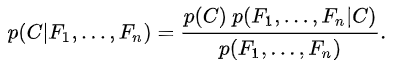
\includegraphics[width=9cm, keepaspectratio]{img/formulabayes}
	\caption{Fórmula de probabilidad de Naive Bayes.}
	\label{fig:formulabayes}
\end{figure}

En la práctica~\cite{machinelearning} solo importa el numerador, puesto que el denominador no depende de C y los valores de Fi son datos, por lo que el denominador será constante. En el numerador es donde se asume que cada Fi es independiente de cualquier otra Fj (siempre que j es distinta de i) cuando estas dependen de C. Esto significa que haciendo estos supuestos, la probabilidad de C teniendo en cuenta las variables clasificatorias puede expresarse como muestra la Figura~\ref{fig:ffinalbayes} donde Z es un factor que depende únicamente de F1 \dots Fn, es decir, constante si los valores de Fi son conocidos.

\begin{figure}
	\centering
	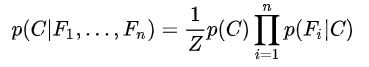
\includegraphics[width=9cm, keepaspectratio]{img/ffinalbayes}
	\caption{Fórmula de final de Naive Bayes.}\label{fig:ffinalbayes}
\end{figure}

Lo que hace el clasificador finalmente es calcular la probabilidad de cada posible clase con las características de entrada y asigna la entrada a esa clase.

\section{Modelo K-NN o K vecinos más cercanos} 
\label{sec:modeloknn}

El modelo de K-NN (\emph{k-nearest neighbors}) o \emph{k} vecinos más cercanos~\cite{knn1,knn2} es un método estadístico de reconocimiento de patrones supervisado. Es un modelo no paramétrico ya que usa directamente los datos de entrenamiento para inferir cada vez la clasificación de una nueva entrada pero sin construir explícitamente un modelo. Lo primero que hace el algoritmo de K-NN es colocar las entradas de entrenamiento en una dimensión de tamaño i, donde i es el número de características. Luego coloca la entrada que queremos clasificar en esta misma dimensión. Después de esto, calcula la distancia a los K puntos más cercanos y en función de la clase de la que tenga más vecinos cerca clasificará la entrada en esa clase. Lo más habitual es seleccionar valores de K pequeños e impares, para evitar los empates. 

\begin{figure}
	\centering
	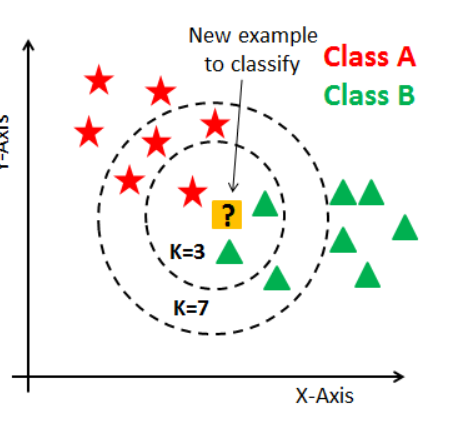
\includegraphics[width=9cm, keepaspectratio]{img/knn}
	\caption{Clasificador K-NN}\label{fig:knn}
\end{figure}


En la Figura~\ref{fig:knn} podemos ver cómo en este caso las características serían dos, una en cada eje y, por tanto, tendríamos tendríamos dos clases. En el caso de utilizar una K con valor 3, asignaría la entrada que estamos evaluando a la clase B. Sin embargo, si tomamos el valor siete para la K, la clasificaría como clase A. Con este ejemplo, nos damos cuenta de que es importante que el valor de K sea pequeño. Este parámetro será uno de los que pueda modificar el usuario en la aplicación web de \texttt{LearningML}.


%%%%%%%%%%%%%%%%%%%%%%%%%%%%%%%%%%%%%%%%%%%%%%%%%%%%%%%%%%%%%%%%%%%%%%%%%%%%%%%%
%%%%%%%%%%%%%%%%%%%%%%%%%%%%%%%%%%%%%%%%%%%%%%%%%%%%%%%%%%%%%%%%%%%%%%%%%%%%%%%%
% DISEÑO E IMPLEMENTACIÓN %
%%%%%%%%%%%%%%%%%%%%%%%%%%%%%%%%%%%%%%%%%%%%%%%%%%%%%%%%%%%%%%%%%%%%%%%%%%%%%%%%

\cleardoublepage
\chapter{Diseño e implementación}

En esta sección veremos cómo se ha llevado a cabo la construcción de los dos nuevos servicios y cómo se ha tenido que reestructurar la aplicación web de \texttt{LearningML}.

\section{Arquitectura antigua de LearningML} 
\label{sec:arquitecturaantigua}

Lo primero que hay que tener claro a la hora de hacer algún cambio en una aplicación web es su estructura.
Por eso vamos a ver cómo funcionaba LearningML antes de realizar el cambio en su forma de trabajar. Hay que tener en cuenta que LearningML está construido por Angular, por lo que esta compuesto por módulos, componentes y servicios. Es importante recordar que antes solo se usaba un algoritmo (redes neuronales) de ahí esta estructura.

Según estaba construido \texttt{LearningML}, en el módulo principal \texttt{AppModule} se cargaba el componente \texttt{ml-model} y el componente \texttt{ml-test-model} uno para construir el modelo y otro para probarlo respectivamente. Estos dos componentes tenían importados a su vez los servicios \texttt{image-classifier} y \texttt{classifier}, uno para crear un modelo de imágenes y otro de texto. El servicio para clasificar texto se llamaba únicamente \texttt{classifier} porque fue el primero que se incorporó cuando Juan David Rodríguez, el co-tutor del proyecto, creó la aplicación web y no sabía si se añadirían más en un futuro.

De manera transversal a todo esto teníamos el servicio \texttt{labeled-data-manager}, que era una especie de ``cajón de sastre" donde se almacenan algunos datos que necesitábamos en los otros servicios y componentes.

Para la parte de test había un solo componente llamado \texttt{ml-test-model} que llamaba a la función \texttt{classify} de \texttt{image-classifier} o a la función  \texttt{run} de \texttt{classifier}, dependiendo de si se estaban clasificando imágenes o textos respectivamente.
En la Figura~\ref{fig:modeloantiguo} se puede ver que contenía cada uno de los servicios nombrados anteriormente.

\begin{figure}
	\centering
	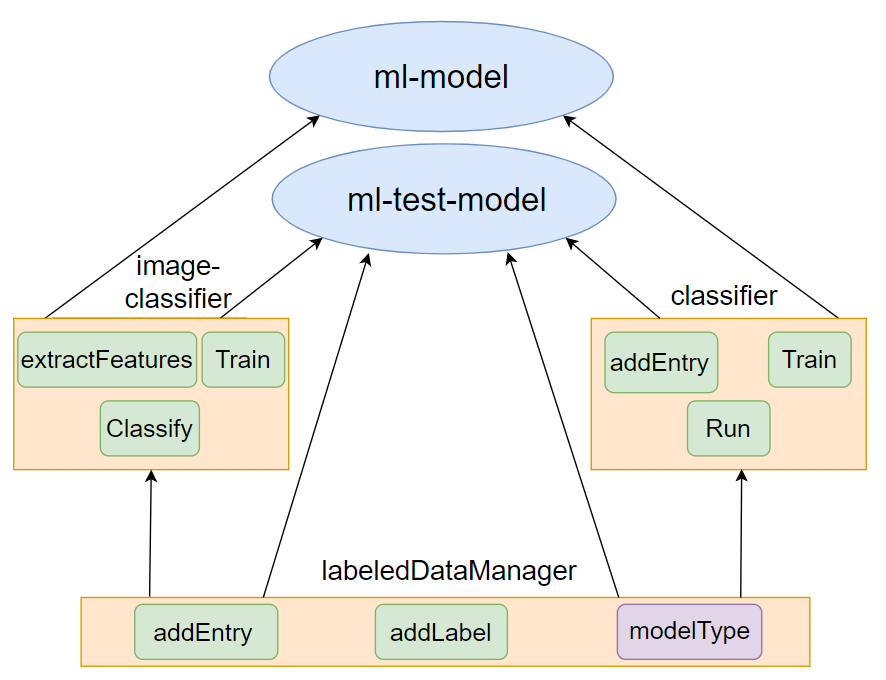
\includegraphics[width=12cm, keepaspectratio]{img/modeloantiguo}
	\caption{Estructura antigua de \texttt{LearningML}. En azul los componentes, en naranja los servicios, en verde las funciones y en morado las variables.}				\label{fig:modeloantiguo}
\end{figure}


\begin{itemize}
  
	\item Labeled-Data-Manager: Era un servicio que se encargaba de guardar los datos en bruto, ya fueran imágenes o textos con la función \texttt{addEntry}. También almacenaba las etiquetas, es decir, las distintas posibles clases a las que podía pertenecer una entrada utilizando la función \texttt{addLabel}. Por último, guardaba el tipo de modelo que se quería construir directamente en la variable \texttt{modelType}. En caso de que cargásemos los datos de un JSON, también es aquí donde se realizaba tanto la carga como la exportación.
 
	\item ImageClassifier: Dentro de este servicio encontrábamos tres funciones principales, \\ \texttt{extractFeature} que se encargaba de transformar las imágenes de entrada en tensores, \texttt{train} que construía el modelo y lo entrenaba y por último \texttt{classify} que evaluaba la imagen de entrada de test y la asignaba a una de las posibles opciones (etiquetas). Dentro de esta última función teníamos que volver a llamar a \texttt{extractFeature} para que transformase la imagen a tensor y poder analizarla.

	\item Classifier: Este servicio lo que hacía era transformar las entradas de texto en bruto en vectores, en esta ocasión se utilizaba la biblioteca BrainText, que es una adaptación que hizo Juanda de la biblioteca Brain.js\footnote{\url{https://brain.js.org/}}. De nuevo, contenía la función \texttt{train} encargada de crear el modelo y entrenarlo y la función \texttt{run}, que sería el equivalente a la función \texttt{classify} del punto anterior, es decir, leía el texto introducido, lo trataba y lo evaluaba y por último determinaba a cuál de los grupos o etiquetas pertenecía.

\end{itemize}

\section{Arquitectura actual de \texttt{LearningML}} 
\label{sec:arquitecturaactual}

Como hemos visto en la sección anterior, tenemos tanto la extracción de características (el proceso de convertir los datos en bruto en un vector que pasar como entrada al constructor del modelo) como la construcción del modelo en el mismo servicio. La idea que tenemos en mente es que por un lado se extraigan las características y por otro lado se genere el modelo independientemente de si estamos clasificando imágenes o texto, ya que al constructor del modelo le entrará un vector sin importar si se ha construido de una forma u otra.\\
Ahora el componente \texttt{ml-model} importa los servicios de \texttt{feature-extraction} y \texttt{ml-algorithm}. Dentro de estos dos servicios, se importan a su vez en el primero \texttt{feature-extractor-image} y \texttt{feature-extractor-text} y en el segundo \texttt{ml-algorithm-image} y \texttt{ml-algorithm-text}.
En el componente \texttt{ml-model} existe la función \texttt{train}, que existía también antes pero llamaba directamente a uno de los dos antiguos servicios, ahora llama a \texttt{feature-extraction} y es este quién elige que servicio usar para extraer el vector dependiendo del tipo de dato. Después llama a \texttt{ml-algorithm} y este servicio decide que algoritmo utilizar para construir el modelo.\\
En la parte de prueba se ha dividido el componente \texttt{ml-test-model} en dos \texttt{ml-test-image} y \texttt{ml-test-text} para imágenes y texto respectivamente. El componente \texttt{ml-test-image} contiene la función \texttt{takeSnapshot} (en caso de que la imagen de prueba sea una foto a través de la cámara) y la función \texttt{onLoaded} (en caso de que la imagen sea un archivo ya existente), en ambos casos, se llama primero a \texttt{feature-extraction} y después a \texttt{ml-algorithm}. En el caso del texto funciona de la misma manera pero solo podemos introducir texto por teclado.\\
El servicio de \texttt{labeled-data-manager} sigue siendo transversal a todos los servicios y componentes, con el único añadido de que ahora guardamos el tipo de algoritmo que vamos a utilizar en la variable \texttt{mlAlgorithm}.
Esta estructura simplifica mucho las cosas y hace que el código sea más fácil de entender y de modificar en caso de que algún día haya que añadir nuevos tipos de datos o nuevos tipos de algoritmos. Hace que las funciones y en general el código sean similares para distintos tipo de datos, además, separa los dos problemas por completo haciéndolos totalmente independientes uno de otro. De nuevo, vamos a ver la Figura~\ref{fig:modelonuevo} para entenderlo mejor.

\begin{figure}
	\centering
	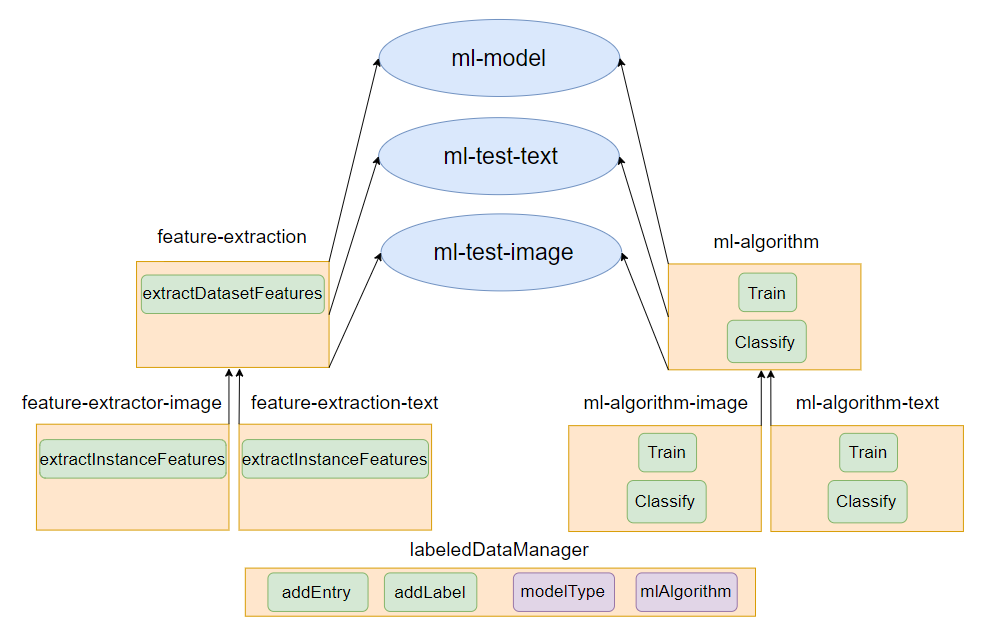
\includegraphics[width=12cm, keepaspectratio]{img/modelonuevo}
	\caption{Estructura nueva de \texttt{LearningML}. En azul los componentes, en naranja los servicios, en verde las funciones y en morado las variables.}					\label{fig:modelonuevo}
\end{figure}

\begin{itemize}
  
	\item Labeled-Data-Manager: Este servicio como ya se ha comentado sigue siendo utilizado en todo el resto de servicios y componentes, con la diferencia de que ahora, además de los datos de etiquetas, datos en bruto de las entradas y tipo de modelo que ya guardaba antes, guarda también el tipo de algoritmo en la variable \texttt{mlAlgorithm}.
 
	\item Feature-Extraction: En este servicio encontramos la función de \texttt{extractDatasetFeatures} que es la encargada de llamar a los otros dos servicios dependiendo de si se quieren extraer características de una imagen o de un texto.
\begin{itemize}
  
	\item Feature-Extractor-Image: Se encarga de extraer las características de las imágenes, es decir, de convertir la imagen en bruto a un tensor. La función que realmente hace esto de obtener el tensor dada una imagen es \texttt{extractInstanceFeatures}. Aunque tiene más funciones para por ejemplo saber que etiqueta corresponde a cada imagen.

	\item Feature-Extractor-Text: Se encarga de extraer las características de los textos, por tanto, con un texto como entrada obtenemos un tensor. De nuevo, para que la arquitectura tenga una estructura coherente, la función recibe el mismo nombre que en el caso de las imágenes \texttt{extractInstanceFeatures}. 
\end{itemize}

	\item ml-Algorithm: Este servicio cuenta con dos funciones principales. \texttt{train} encargada de elegir a que sub-servicio llamar dependiendo del algoritmo que se quiere utilizar. Y la función \texttt{classify} que de nuevo, elige que sub-servicio utilizar en función del algoritmo.
\begin{itemize}
  
	\item ml-Algorithm-knn: Cuenta con dos funciones que son las que llama el servicio que esta por encima para entrenar (\texttt{train}) o evaluar  (\texttt{classify}) una entrada en el caso de que el algoritmo elegido por el usuario sea K-NN.

	\item ml-Algorithm-bayes: Cuenta con las mismas funciones que K-NN pero en este caso construye o evalúa un clasificador utilizando el algoritmo de Naive Bayes.
\end{itemize}


\end{itemize}

Finalmente, recalcar que esta estructura si se utiliza correctamente permite añadir un nuevo tipo de dato o de clasificador únicamente creando los nuevos servicios. Debemos tener en cuenta que estos nuevos servicios para que encajen con lo que ya hay deben tener al menos las mismas funciones que los ya existentes, ya que son a las que llaman los servicios superiores. De esta manera, sin apenas tocar los servicios superiores (solo habría que añadir en el punto donde se elije el tipo de dato a extraer o el tipo de modelo, la opción de elegir lo nuevo que hayamos creado) podemos implementar nuevas funcionalidades en un futuro de manera más limpia y sencilla.



\section{Adaptar la interfaz} 
\label{sec:interfaz}

En este caso, lo primero que se hizo fue añadir en la interfaz gráfica la opción de que el usuario pudiera elegir que tipo de algoritmo utilizar, Naive Bayes, K-NN o redes neuronales. Para ello hay que modificar el archivo \texttt{ml-model.component.html} como se puede ver en la Figura~\ref{fig:desplegable} añadiendo un desplegable \texttt{select} con las tres opciones que tenemos ahora. Como podemos ver en la primera línea, este desplegable solo aparecerá en caso de que tengamos activado el \texttt{LearningML} avanzado, si no tenemos este modo activado no nos dejará elegir el tipo de modelo y utilizará redes neuronales.\\

\begin{figure}
	\centering
	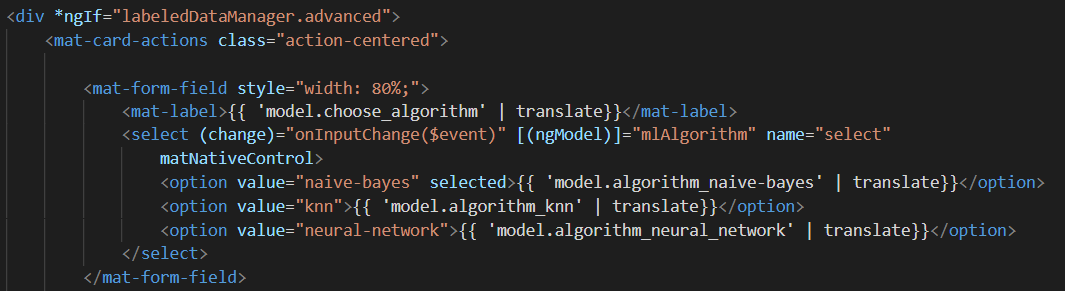
\includegraphics[width=12cm, keepaspectratio]{img/desplegable}
	\caption{Parte de código encargada de crear el desplegable que muestra los tipos de modelo que puede elegir el usuario}									\label{fig:desplegable}
\end{figure}

Dependiendo de la opción que elijamos en el desplegable, nos dejará modificar unos parámetros u otros. 
En el caso de K-NN nos deja elegir el número de vecinos que queremos tener en cuenta a la hora de clasificar, es decir, el valor de \emph{K}. Esto se hace en el mismo archivo en la parte que se muestra en la Figura~\ref{fig:nvecinosknn}. En la primera linea se comprueba si el algoritmo es K-NN para ver si se muestra esto o no, y en la tercera otorgamos el valor mínimo y máximo del deslizable así como el intervalo entre un valor y otro, en este caso 1. También recogemos su valor en \texttt{params.knn.k} para después poder utilizarlo.

\begin{figure}
	\centering
	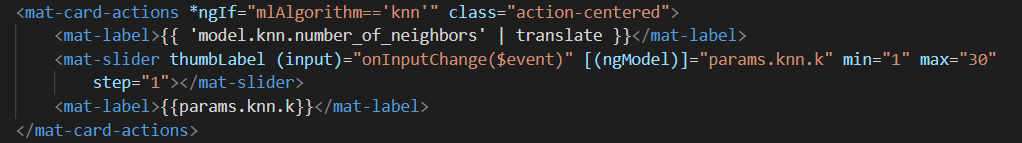
\includegraphics[width=12cm, keepaspectratio]{img/nvecinosknn}
	\caption{Parte de código encargada de recoger el valor de K en el algoritmo KNN}				
        \label{fig:nvecinosknn}
\end{figure}

\section{Datos de entrada} 
\label{sec:datosdeentrada}

A la hora de crear un nuevo servicio, tenemos que tener claro cómo vienen los datos de entrada y cómo podemos trabajar con ellos. Como ya hemos comentado antes, en el servicio \texttt{feature-extraction} se llama al servicio correspondiente para extraer las entradas del clasificador a partir de los datos en bruto. Estos datos en bruto tienen el aspecto que vemos en la Figura~\ref{fig:datosenbruto}. Como vemos consta de tres pares de datos clave-valor, uno por cada etiqueta y las entradas que pertenecen a ella.

\begin{figure}
	\centering
	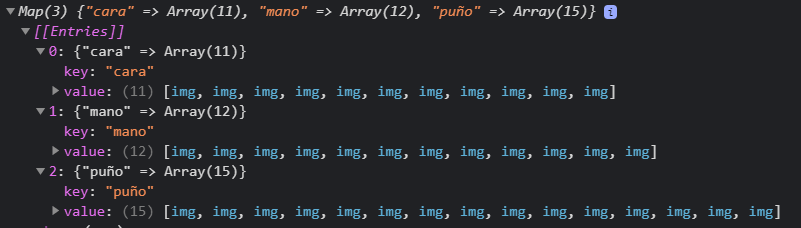
\includegraphics[width=12cm, keepaspectratio]{img/datosenbruto}
	\caption{Datos de entrada sin tratar}				
	\label{fig:datosenbruto}
\end{figure}

Ahora vamos a ver en que se transforman estos datos para ver que va a recibir nuestro clasificador. La función \texttt{train} de nuestro clasificador que se llamará en el servicio \texttt{ml-algorithm} tendrá como entrada \texttt{features}. Este objeto se compone de tres items:

\begin{itemize}
  
	\item \texttt{text\_labels}: Es simplemente un array con los nombres de las etiquetas, para después poder equiparar los datos del tensor con la realidad. En la Figura~\ref{fig:textlabels} tenemos la estructura del dato.

\begin{figure}
	\centering
	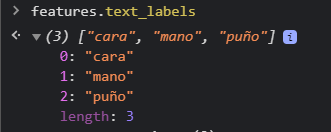
\includegraphics[width=12cm, keepaspectratio]{img/textlabels}
	\caption{Estructura de text\_labels}				
	\label{fig:textlabels}
\end{figure}

	\item \texttt{tensor\_labels}: Es un tensor en el que se guardan las etiquetas codificadas como tres números. En este caso que tenemos en total 38 entradas y tres etiquetas, tendrá 38 arrays de tamaño tres. Cuando el array tenga valor [1,0,0] significará que esa entrada pertenece a la primera etiqueta, en el caso de que tome el valor [0,1,0] pertenecerá a la segunda etiqueta y por último, si toma el valor [0,0,1] será de la tercera etiqueta. Podemos ver el aspecto de este dato en la Figura~\ref{fig:tensorlabels}.

\begin{figure}
	\centering
	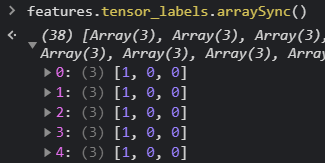
\includegraphics[width=12cm, keepaspectratio]{img/tensorlabels}
	\caption{Estructura de tensor\_labels}				
	\label{fig:tensorlabels}
\end{figure}
	
	\item \texttt{tensor\_inputs}: Es un tensor en el que se encuentran las características de cada entrada, en el caso de las imágenes que es lo que vamos a tratar en el ejemplo, utilizamos 1024 características y tenemos 38 entradas. Cada entrada por tanto tendrá un vector de 1024 posiciones y cada posición tendrá el valor de una característica. La estructura de este dato la podemos ver en la Figura~\ref{fig:tensorinputs}

\begin{figure}
	\centering
	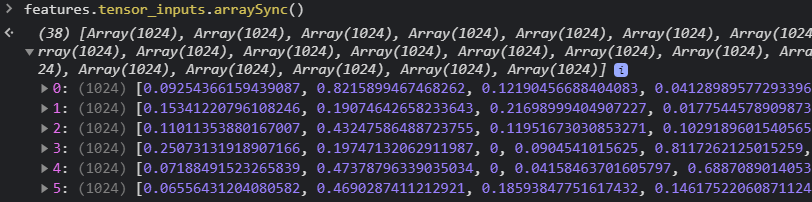
\includegraphics[width=12cm, keepaspectratio]{img/tensorinputs}
	\caption{Estructura de tensor\_inputs}				
	\label{fig:tensorinputs}
\end{figure}


\end{itemize}

\section{Crear el clasificador de K-NN} 
\label{sec:knn}

Para crear el clasificador de K-NN lo primero es tener claro cómo funciona para poder pasarlo a lenguaje de programación. Vamos a verlo con un ejemplo, en la Figura~\ref{fig:ejemploknn} podemos ver que tenemos tres grupos, lo que para nosotros serán las etiquetas y dos características, la altura y el peso, que en nuestro caso serán 1024. 

\begin{figure}
	\centering
	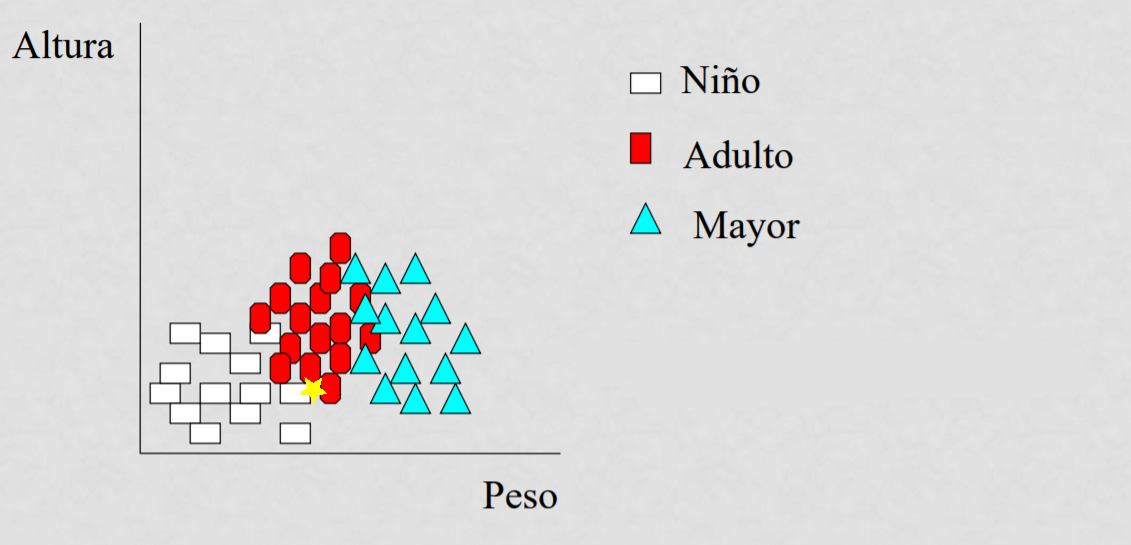
\includegraphics[width=12cm, keepaspectratio]{img/ejemploknn}
	\caption{Creación del modelo de K-NN}				
	\label{fig:ejemploknn}
\end{figure}

El modelo coloca los datos de entrenamiento en el espacio y después a la hora de evaluar, según las características que recibe, sitúa el dato de evaluación. Por último, mirará los K vecinos más cercanos, en este caso vamos a suponer 3, y asignará la nueva entrada al grupo del que tenga un mayor número de vecinos cercanos, en este caso tiene dos vecinos rojos y uno blanco, por lo que será clasificado como adulto.

\subsection{Función Train} 
\label{sec:funciontrainknn}

Tanto esta función como la siguiente se pueden encontrar en el archivo /learningml-editor-develop/src/app/services/mlAlgorithms/ml-algorithm-knn.ts.

Por cómo funciona la biblioteca que vamos a utilizar de TensorFlow, necesitamos en primer lugar construir el modelo con la función  \texttt{knnClassifier.create()} (previamente hemos importado la biblioteca como knnClassifier). Lo que hará este objeto será ir situando las entradas como los puntos que hemos visto en el ejemplo, pero en este caso el espacio será de 1024 dimensiones. Este modelo funciona de tal forma que tenemos que ir añadiendo entradas de entrenamiento con la función \texttt{.addExample()}. Esta función tiene que recibir dos parámetros, por un lado debe tener las características de una entrada en un tensor y por otro la etiqueta a la que pertenece indicada como un número. Podemos ver las estructuras de entrada en la Figura~\ref{fig:entradasclasificadorknn}.

\begin{figure}
	\centering
	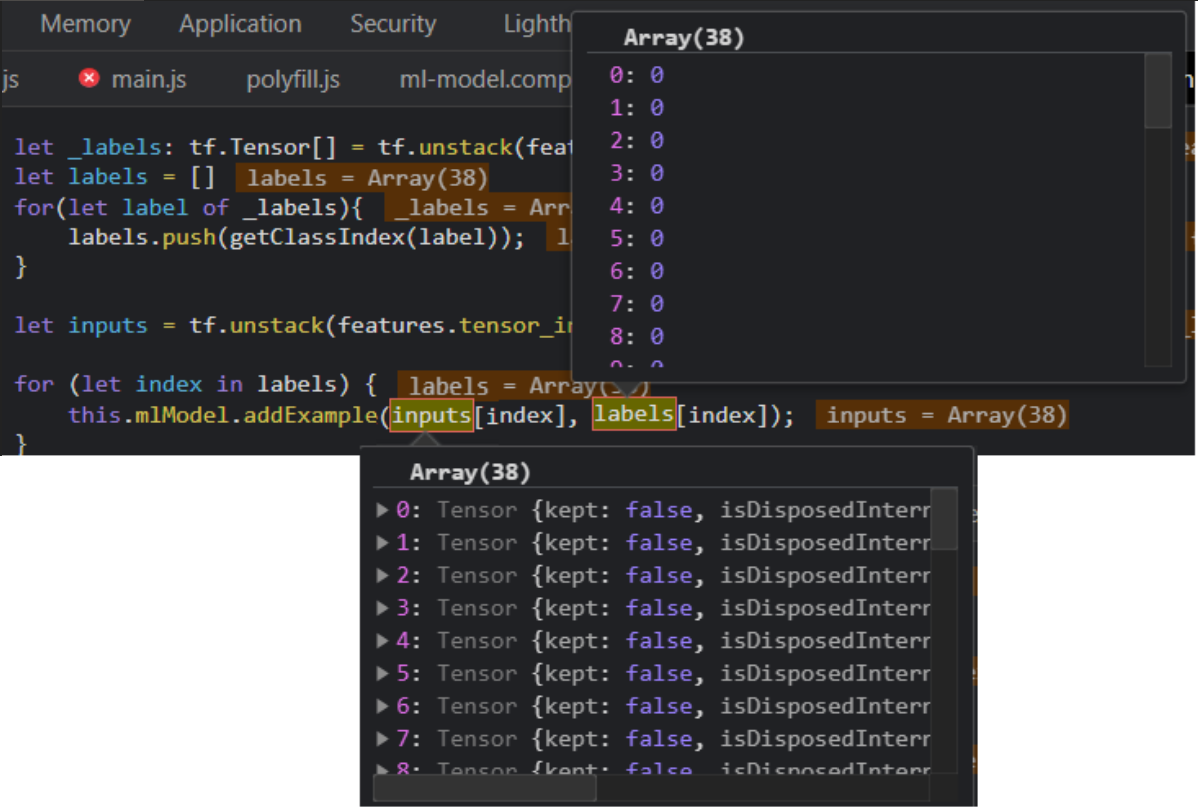
\includegraphics[width=12cm, keepaspectratio]{img/entradasclasificadorknn}
	\caption{Estructura de los datos de entrada al clasificador de K-NN}				
	\label{fig:entradasclasificadorknn}
\end{figure}

Vamos a ver cómo conseguir este tipo de dato para cada caso:

\begin{itemize}
	\item Características: En este caso es sencillo, ya que solamente tenemos que deshacer el vector que tenemos en \texttt{tensor\_inputs} y obtener un vector por cada característica. TensorFlow cuenta con la función \texttt{unstack} que hace precisamente eso.
\begin{verbatim}
let inputs = tf.unstack(features.tensor_inputs);
\end{verbatim}	
	\item Etiquetas: Para obtener esta variable también tenemos que deshacer el vector de etiquetas \texttt{tensor\_labels} en un tensor para cada entrada (estos tensores se guardan en la variable \texttt{\_labels}). Después de esto tenemos que remplazar el array de tres posiciones que teníamos por un solo número, de eso se encarga la función auxiliar  \texttt{getClassIndex} que obtiene para cada array su numero correspondiente, en este caso al array [1,0,0] le corresponderá el valor 0, al array [0,1,0] el valor 1 y al array [0,0,1] el valor 2. Este formato de etiquetas final se guarda en la variable \texttt{labels}.
\end{itemize}

Por último, queda construir un bucle que vaya añadiendo todos los ejemplos, es decir, que recorra las posiciones de los dos arrays que tenemos pasándoselas como argumentos a la función \texttt{addExample} que tiene el modelo (objeto) que hemos creado al principio.

\subsection{Función Classify} 
\label{sec:funcionclassifyknn}

Una vez hemos construido y entrenado el modelo, queda crear la función para que clasifique una entrada dada. En este paso colocará la entrada en el espacio de dimensión 1024 con el resto de ejemplos ya colocados y verá cuáles son los K vecinos más cercanos. Después clasificará nuestra entrada como la etiqueta de la cual tenga más vecinos cercanos, es decir, si nos fijamos en los tres vecinos más cercanos y dos son del tipo adulto y uno del tipo niño clasificará la entrada como adulto. En este caso tenemos la función \texttt{.predictClass} a la que le tenemos que pasar un tensor con las características de la entrada y el valor del parámetro K. En este caso es inmediato, ya que ambas variables las tenemos. Sin embargo, esta función devuelve una probabilidad para cada etiqueta, que si recordamos, ahora valen 0, 1 o 2. Debido a esto, tenemos que recorrer el array que nos ha devuelto con las probabilidades ordenadas, es decir, el primer dato corresponde a la primera etiqueta asignando a cada nombre de etiqueta (recordar que lo guardábamos en \texttt{text\_labels}) su probabilidad. Estos datos se guardan en la variable \texttt{results} que tiene el aspecto que podemos ver en la Figura~\ref{fig:resultsknn}; se trata de un array en el que cada elemento es otro array en el que la primera posición es el nombre de la etiqueta y la segunda la probabilidad de la misma. Por último, ordenamos la variable antes de devolverla al servicio superior (\texttt{ml-algorithm}) donde se llama a esta función.

\begin{figure}
	\centering
	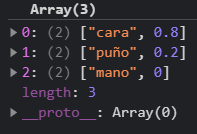
\includegraphics[width=8cm, keepaspectratio]{img/resultsknn}
	\caption{Variable con la probabilidad correspondiente a cada etiqueta.}				
	\label{fig:resultsknn}
\end{figure}

\section{Crear el clasificador de Naive Bayes} 
\label{sec:naivebayes}

De nuevo, vamos a ver un ejemplo para tener presente que es lo que tenemos que hacer e ir equiparándolo a los datos del ejemplo con los datos que tenemos y los que queremos conseguir. Veamos el ejemplo que se muestra en el libro de S. Marsland~\cite{machinelearning}. Tenemos una serie de datos con su salida correspondiente (ver Tabla~\ref{fig:tablabayes}).
En este caso tendríamos tres características: si hay entregas de ejercicios pendientes, si hay una fiesta y si la persona se siente vaga o no ese día. Dependiendo de esto podrá hacer cuatro actividades distintas, salir de fiesta, estudiar, irse al bar o ver la televisión. 
Para nosotros, las características, son 1024 y las actividades posibles serían nuestras etiquetas. Otro parámetro a tener en cuenta es la cantidad de valores que puede tomar cada etiqueta, en nuestro caso son prácticamente infinitos, por lo que una de las cosas que haremos será agruparlos en cinco posibles valores por etiqueta. 

\begin{figure}
	\centering
	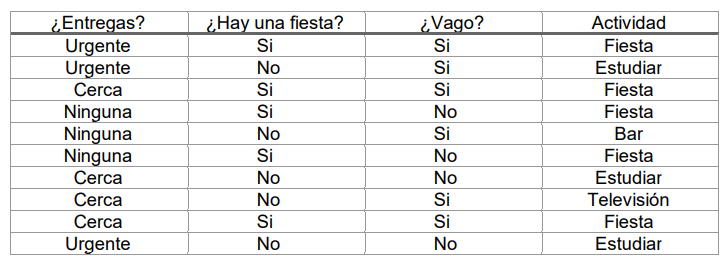
\includegraphics[width=12cm, keepaspectratio]{img/tablabayes}
	\caption{Tabla con los datos de ejemplo de Naive Bayes.}			
	\label{fig:tablabayes}
\end{figure}



\subsection{Función Train} 
\label{sec:funciontrainbayes}

Tanto esta función como la siguiente se pueden encontrar en el archivo /learningml-editor-develop/src/app/services/mlAlgorithms/ml-algorithm-naive-bayes.ts.

Lo primero de todo es hacer un proceso similar al que hicimos en K-NN, en este caso para guardar en un array de dos dimensiones todas las entradas y todas las características de cada una. Es decir existirá un array que tendrá tantos arrays como ejemplos tengamos, y cada ejemplo a su vez es un array de los valores de las 1024 características (o 512 en el caso de los textos), ya que vamos a trabajar con imágenes para ver cómo funciona.

Para saber cuáles son los datos que tenemos que calcular en esta función debemos tener claro el objetivo final. Lo que hay que hacer es calcular la posibilidad de las cuatro posibles salidas dada una entrada, es decir un array de 1024 características. Eso se hace con los cálculos que se muestran en la Figura~\ref{fig:probabilidadbayes}. 

\begin{figure}
	\centering
	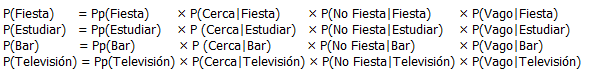
\includegraphics[width=12cm, keepaspectratio]{img/probabilidadbayes}
	\caption{Cálculo de probabilidad de cada salida en Naive Bayes.}			
	\label{fig:probabilidadbayes}
\end{figure}

La primera columna de cada fila es sencilla, pues únicamente tenemos que dividir el numero de veces que tenemos una etiqueta entre el total de entradas que hay. Para ello, guardaremos en un array las veces que tenemos cada etiqueta, además con la longitud de este array podremos saber también el número de etiquetas que hay. 
El resto de columnas es la parte complicada, para ver de dónde vienen estos valores, vamos a ver primero la tabla de contingencia de la característica vago en la Figura~\ref{fig:tablavago}. 

\begin{figure}
	\centering
	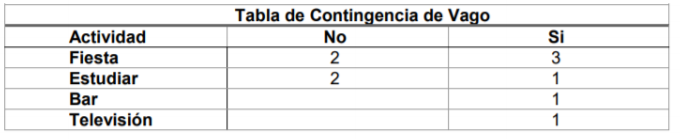
\includegraphics[width=12cm, keepaspectratio]{img/tablavago}
	\caption{Tabla de contingencia de la característica \emph{vago}.}			
	\label{fig:tablavago}
\end{figure}

Con esta tabla podemos calcular la probabilidad de una etiqueta dado un valor de la característica. Para entender esto mejor vamos a ver el ejemplo, si ahora se introdujese una entrada en la que hay entregas de ejercicios cerca, no hay fiestas y me siento vago, la probabilidad de la etiqueta fiesta condicionada a que me siento vago sería de 3/5 ya que de las cinco veces que la salida era fiesta en los ejemplos, en tres me sentía vago. Esto es la clave de todo, cuesta un poco entenderlo al principio, pero es cómo funcionan las probabilidades condicionadas.

Sigamos con el ejemplo, vamos a verlo para una etiqueta, pero sería de la misma forma con todas. Una vez tenemos los valores de las probabilidades de una etiqueta condicionadas con el valor de una característica, lo que tenemos que hacer es multiplicar estas probabilidades entre sí, es decir, las de todas las características y multiplicarlas también por la probabilidad de la etiqueta que en el caso de fiesta es 5/10. Por tanto la probabilidad de la etiqueta fiesta dada la entrada de características que hemos mencionado antes sería la que vemos en la Figura~\ref{fig:probabilidadesbayes}. 

\begin{figure}
	\centering
	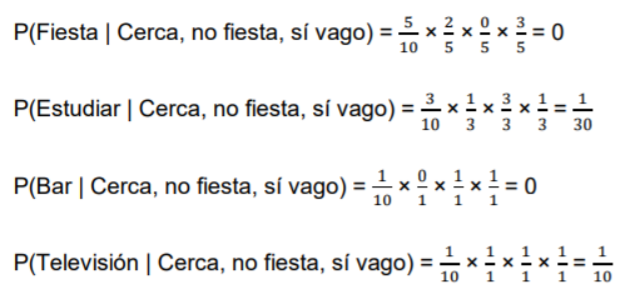
\includegraphics[width=12cm, keepaspectratio]{img/probabilidadesbayes}
	\caption{Probabilidades de las etiquetas fiesta y televisión.}			
	\label{fig:probabilidadesbayes}
\end{figure}

En esta misma imagen tenemos también la probabilidad de la etiqueta televisión, que en este caso es la mayor, ya que aunque su primera columna es 1/10 por que solo teníamos una entrada de ejemplo con esa etiqueta, como las tres características tenían exactamente esos valores, sale la probabilidad más alta de las cuatro.

Viendo el ejemplo, es fácil darse cuenta de que estas probabilidades van a ser muy bajas cuando tengamos 1024 características, pues estaremos multiplicando 1024 veces (recordar que también hay que multiplicar por la probabilidad simple de la etiqueta) números menores que uno, o uno en el mejor de los casos.
También es muy posible que para cierta etiqueta alguna característica nunca haya tenido el valor introducido en la entrada de evaluación y si es así esta etiqueta automáticamente valdrá 0, para evitar esto, cuando esto ocurre no se tiene en cuenta esa probabilidad. De igual forma, para intentar evitar números muy pequeños, como ya se ha comentado antes, se han dado 5 valores posibles a cada etiqueta.

Vamos a ver cómo pasar todo esto a código, lo primero que se ha hecho ha sido transponer el array de entradas, para de esta manera tener un array en el que cada posición es una etiqueta con todos sus valores en las distintas entradas, es decir, será un array de 1024 en el que en la primera posición tendremos un array con todos los valores de la primera característica. Una vez tenemos esto, toca normalizar los valores entre 0 y 100. Podemos ver el array en la imagen 
~\ref{fig:caracteristicasnormalizadas}. Lo que vemos en la imagen serían los valores para las primeras 4 características (primera fila todos los valores de la primera característica para cada entrada de ejemplo), tenemos 60 valores para cada una porque se han introducido esas entradas.

\begin{figure}
	\centering
	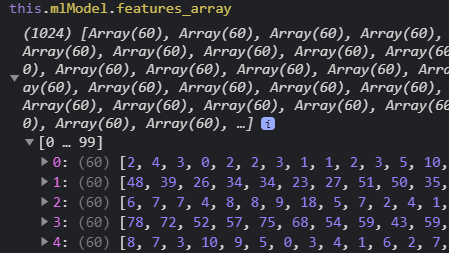
\includegraphics[width=8cm, keepaspectratio]{img/caracteristicasnormalizadas}
	\caption{Características después asignar valores según rango.}			
	\label{fig:caracteristicasnormalizadas}
\end{figure}

En el siguiente paso agruparemos los valores de la siguiente forma, los que estén entre 0 y 19 en un 0, entre 20 y 39 en un 1, entre 40 y 59 en un 2, entre 60 y 79 en un 3 y entre 79 y 100 en un 4. Esto se hace directamente en el momento que contamos las veces que esta cada valor. Podemos ver la estructura y los valores del array en la Figura~\ref{fig:vecesvalor}. Si vemos la función en la Figura~\ref{fig:funcioncontador} vemos que lo que hace es dependiendo del valor de la característica, aumenta un contador u otro. Este es un array tridimensional en el que el primer índice es la etiqueta, el segundo es la característica y el tercero el valor de la característica, entonces en cada una de estas posiciones, se guarda las veces que esta ese valor en esa característica dada esa etiqueta.

\begin{figure}
	\centering
	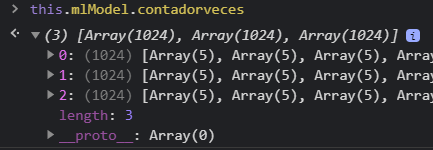
\includegraphics[width=8cm, keepaspectratio]{img/vecesvalor}
	\caption{Número de veces que está un valor para una característica dada una etiqueta.}			
	\label{fig:vecesvalor}
\end{figure}


\begin{figure}
	\centering
	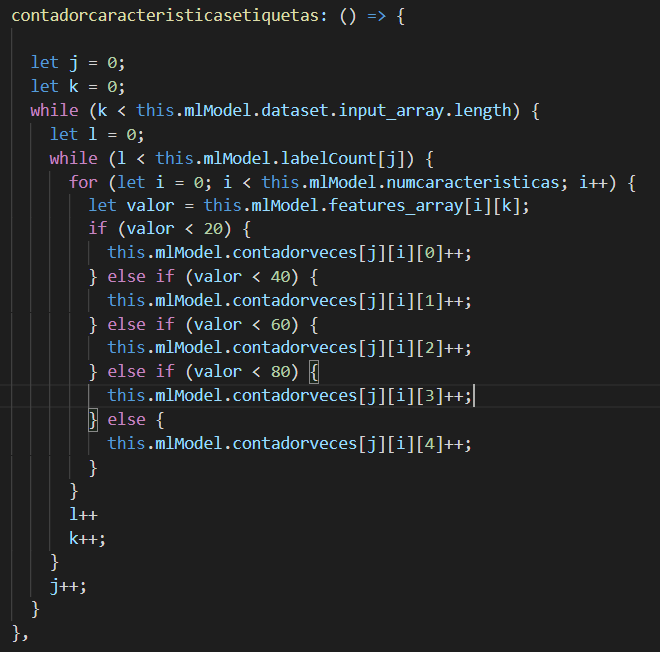
\includegraphics[width=8cm, keepaspectratio]{img/funcioncontador}
	\caption{Función que rellena el array tridimensional con las veces que esta cada valor.}			
	\label{fig:funcioncontador}
\end{figure}

Por último, nos queda dividir el número de veces que esta cada valor entre el número de veces que esta la etiqueta a la que pertenece, es decir, necesitamos recorrer el array anterior dividiendo entre un número u otro dependiendo de la etiqueta. El resultado lo tenemos en la Figura~\ref{fig:probabilidadescalculadas}

\begin{figure}
	\centering
	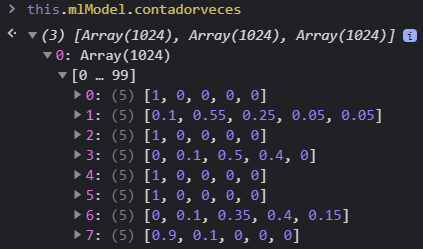
\includegraphics[width=8cm, keepaspectratio]{img/probabilidadescalculadas}
	\caption{Array con las probabilidades de cada valor de cada característica dada una etiqueta.}			
	\label{fig:probabilidadescalculadas}
\end{figure}


\subsection{Función Classify} 
\label{sec:funcionclassifybayes}

Para crear esta función debemos tener en cuenta que necesitamos devolver las probabilidades de cada etiqueta, por tanto, necesitaremos recorrer el array tridimensional buscando la probabilidad condicionada de cada valor de cada característica de entrada para cada una de las etiquetas posibles. Además, también calcularemos la primera fracción y será en esta variable donde iremos acumulando el resultado de todas las multiplicaciones para luego meterlo en otra la cual será el array que devolveremos con las probabilidades de cada etiqueta. Todo esto se hace en la función que se puede ver en la función~\ref{fig:probabilidadesetiquetasbayes}. Si nos fijamos, como se comentó en algún apartado anterior, para intentar obtener resultados legibles y no un 0, cuando alguna de estas probabilidades a multiplicar es 0, no se hace. Además, el una vez tenemos los 3 resultados los intentamos normalizar entre 0 y 1, pero de todas formas, al ser tantas operaciones y números menores que 1, los resultados son extremadamente pequeños como veremos en el capítulo de experimentos y validación.

\begin{figure}
	\centering
	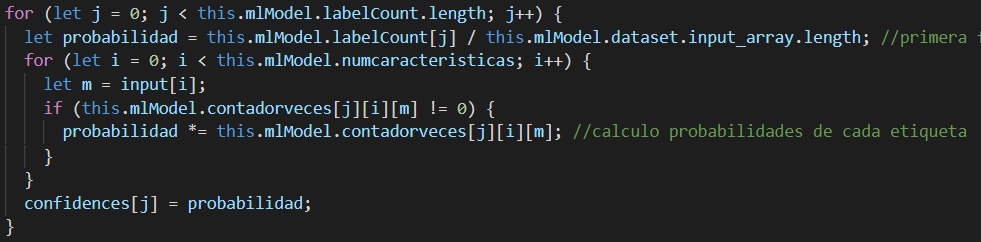
\includegraphics[width=8cm, keepaspectratio]{img/probabilidadesetiquetasbayes}
	\caption{Función que calcula las probabilidades de cada etiqueta en Bayes.}			
	\label{fig:probabilidadesetiquetasbayes}
\end{figure}



%%%%%%%%%%%%%%%%%%%%%%%%%%%%%%%%%%%%%%%%%%%%%%%%%%%%%%%%%%%%%%%%%%%%%%%%%%%%%%%%
%%%%%%%%%%%%%%%%%%%%%%%%%%%%%%%%%%%%%%%%%%%%%%%%%%%%%%%%%%%%%%%%%%%%%%%%%%%%%%%%
% EXPERIMENTOS Y VALIDACIÓN %
%%%%%%%%%%%%%%%%%%%%%%%%%%%%%%%%%%%%%%%%%%%%%%%%%%%%%%%%%%%%%%%%%%%%%%%%%%%%%%%%

\cleardoublepage
\chapter{Experimentos y validación}

En esta sección vamos a realizar algunas comprobaciones para ver si los clasificadores construidos funcionan correctamente o no. Para comprobar el funcionamiento del clasificador, en ambos casos (K-NN y Naive Bayes), cabe destacar que cuanto mayor sea el conjunto de entrenamiento mejor serán los resultados.

\section{Prueba del clasificador de K-NN} 
\label{sec:pruebaknn}

Hemos creado un modelo con tres clases (cara, mano y puño) y en el que para cada clase hemos añadido 11, 12 y 15 fotos respectivamente, aunque lo ideal sería añadir el mismo número de fotos en cada etiqueta de esta manera podemos ver su funcionamiento cuando la situación no es óptima. En la figura~\ref{fig:fotosentrada} podemos ver las entradas. Después de esto, elegimos el clasificador de K-NN y el número de vecinos a tener en cuenta para la clasificación (valor del parámetro K) y pulsamos el botón de aprender a reconocer imágenes.

\begin{figure}
	\centering
	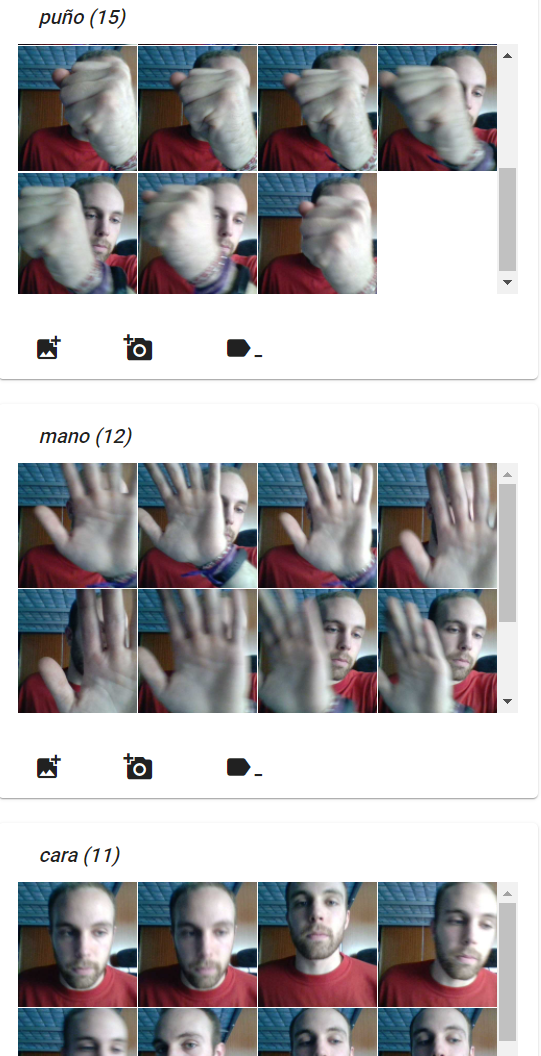
\includegraphics[width=9cm, keepaspectratio]{img/fotosentrada}
	\caption{Elementos de entrada para el entrenamiento del clasificador.}			
	\label{fig:fotosentrada}
\end{figure}

Ahora en la sección de la derecha vamos a hacer (o seleccionar del ordenador) una foto para que la clasifique el modelo. Vamos a comenzar primero con utilizar una entrada de la clase cara y ver que clase se le asigna. Figura~\ref{fig:testcaraknn}. Como podemos ver debajo de la imagen nos muestra el porcentaje de que la entrada evaluada pertenezca a una clase u otra, en este caso ha acertado completamente ya que nos indica un 100\% en la etiqueta cara. Se han hecho varias comprobaciones más con imágenes de la clase cara y funciona correctamente.

\begin{figure}
	\centering
	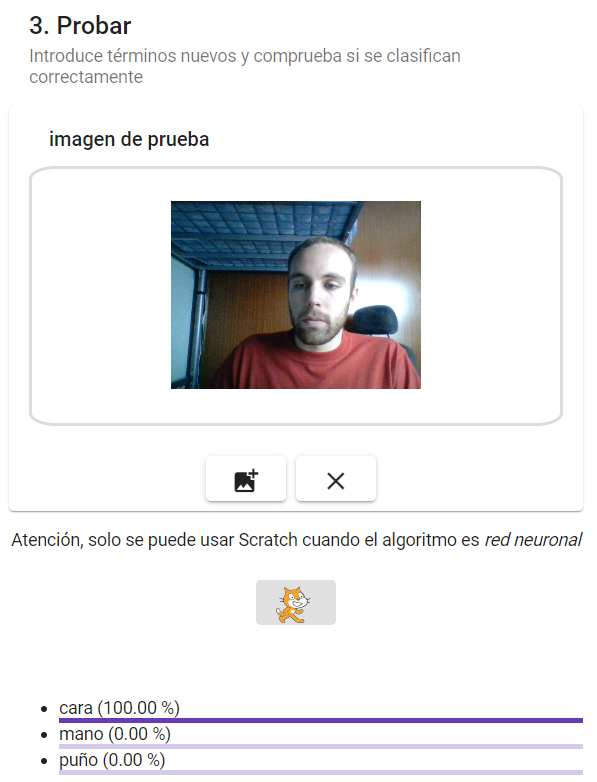
\includegraphics[width=9cm, keepaspectratio]{img/testcaraknn}
	\caption{Imagen de test de la clase cara para el clasificador KNN.}			
	\label{fig:testcaraknn}
\end{figure}

Vamos ahora a comprobar que ocurre si introducimos la imagen de una mano. Figura~\ref{fig:testmanoknnbien}. En este caso si asigna correctamente la imagen a la etiqueta que le corresponde, sin embargo, probando algunas veces más (Figura~\ref{fig:testmanoknnmal}) nos damos cuenta de que, aunque si se clasifique bien la imagen ya que el mayor porcentaje sigue siendo de la clase mano, comienza a tener algún porcentaje del tipo puño. Estos porcentajes, van a ser siempre múltiplos de 20 debido a que hemos elegido un parámetro K con valor 5, por lo que tendrá 1, 2, 3, 4 o 5 vecinos de una clase que se corresponderán con un 20, un 40, un 60, un 80 o un 100 por cien respectivamente. Teniendo esto en cuenta, en el caso de la Figura~\ref{fig:testmanoknnmal} que tiene un 60 \% de mano, querrá decir que 3 de los 5 vecinos más cercanos son de la clase mano y los otros 2 (40\%) son de la clase puño. Podemos observar, que pese a ser imágenes en las que puede haber algo más de confusión, sigue funcionando correctamente ya que el mayor porcentaje sigue siendo de la etiqueta correcta.

\begin{figure}
	\centering
	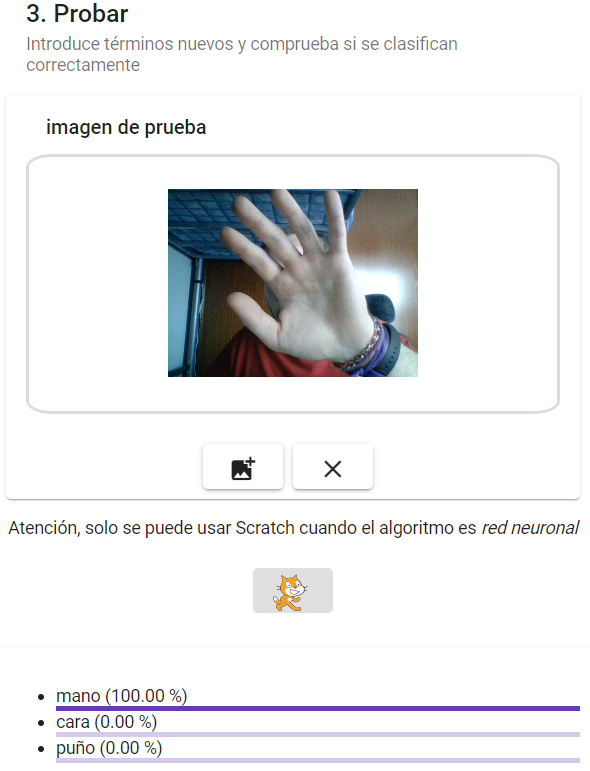
\includegraphics[width=9cm, keepaspectratio]{img/testmanoknnbien}
	\caption{Imagen de test de la clase mano para el clasificador KNN (1).}			
	\label{fig:testmanoknnbien}
\end{figure}

\begin{figure}
	\centering
	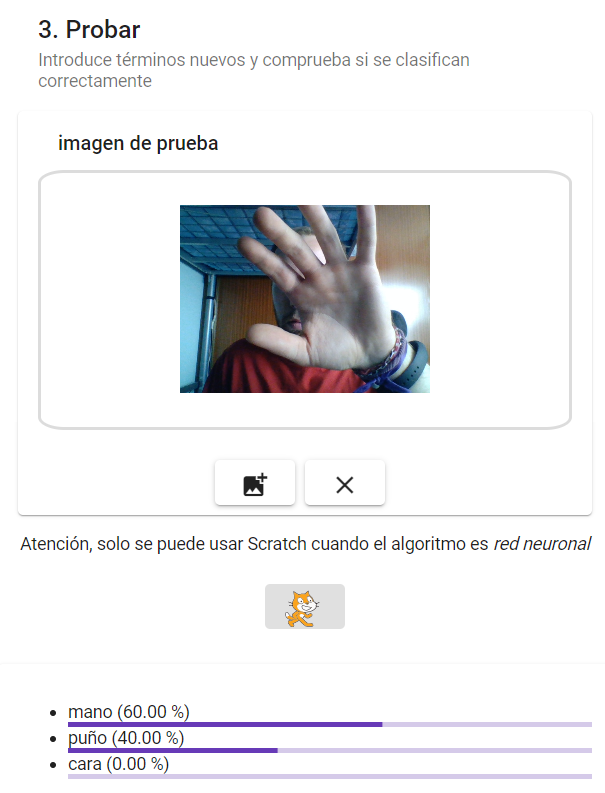
\includegraphics[width=9cm, keepaspectratio]{img/testmanoknnmal}
	\caption{Imagen de test de la clase mano para el clasificador KNN (2).}			
	\label{fig:testmanoknnmal}
\end{figure}

Por último queda evaluar la clase puño. De nuevo ocurre como con la clase mano, en algunos casos nos devuelve un porcentaje del 100\% para la clase correcta (Figura~\ref{fig:testpunoknnbien}) y en otros tiene cierto porcentaje de la clase mano (Figura~\ref{fig:testpunoknnmal}). En este caso podemos ver que tiene un 80\% en la etiqueta puño (4 de los vecinos más cercanos son de la clase puño) y un 20 \& de la etiqueta mano (uno de los cinco vecinos más cercanos pertenece a la clase mano). A pesar de esto, podemos decir que funciona correctamente ya que el mayor porcentaje es para la clase correcta.

\begin{figure}
	\centering
	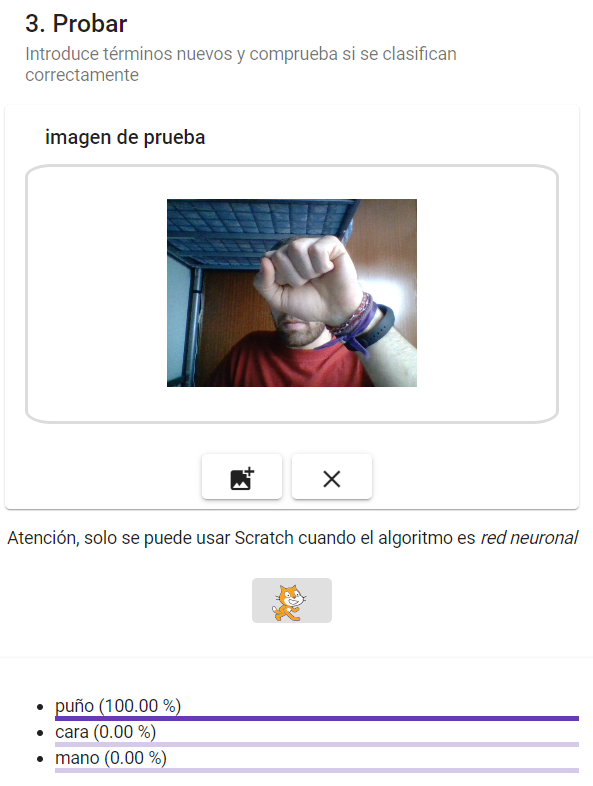
\includegraphics[width=9cm, keepaspectratio]{img/testpunoknnbien}
	\caption{Imagen de test de la clase puño para el clasificador KNN (1).}			
	\label{fig:testpunoknnbien}
\end{figure}

\begin{figure}
	\centering
	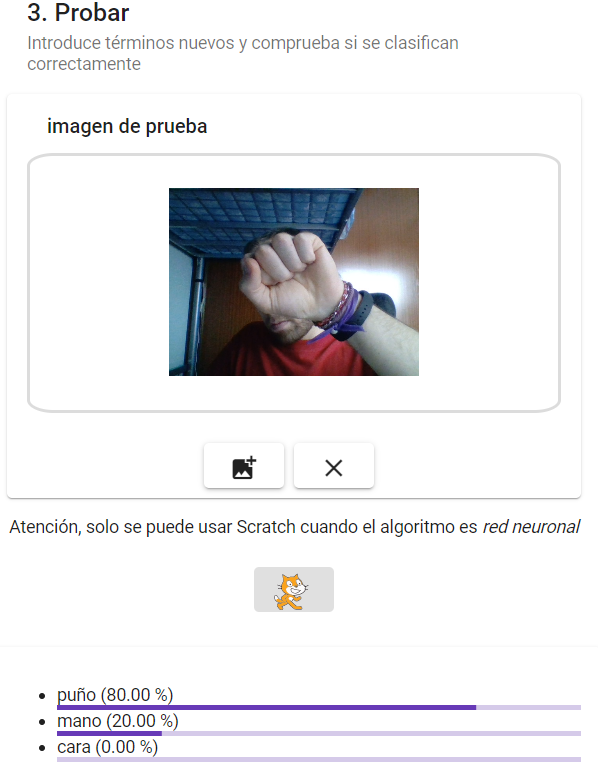
\includegraphics[width=9cm, keepaspectratio]{img/testpunoknnmal}
	\caption{Imagen de test de la clase puño para el clasificador KNN (2).}			
	\label{fig:testpunoknnmal}
\end{figure}



\section{Prueba del clasificador de Naive Bayes} 
\label{sec:pruebabayes}

Como ya se ha comentado en algún punto anterior, por cómo funciona este algoritmo las probabilidades obtenidas son muy pequeñas. Para este ejemplo se han utilizado los mismos datos de entrenamiento y de test que en el caso de K-NN aprovechando que podemos descargar el modelo con los datos de entrenamiento en formato JSON y guardando las imágenes que hicimos para el test.\\
Para el test de cara obtenemos los datos que vemos en la Figura~\ref{fig:bayestestcara}, tenemos los datos de la variable y los que se muestran al usuario. El valor de la variable para la primera etiqueta que sería cara tiene un valor por 10 elevado a menos 300, lo que es infinitamente pequeño. Para las otras etiquetas nos muestra un 0 por el mismo motivo, ya que, matemáticamente, si recordamos la condición que teníamos en el bucle de solo utilizar probabilidades distintas de 0, nunca serán 0 por muy pequeñas que sean.

\begin{figure}
	\centering
	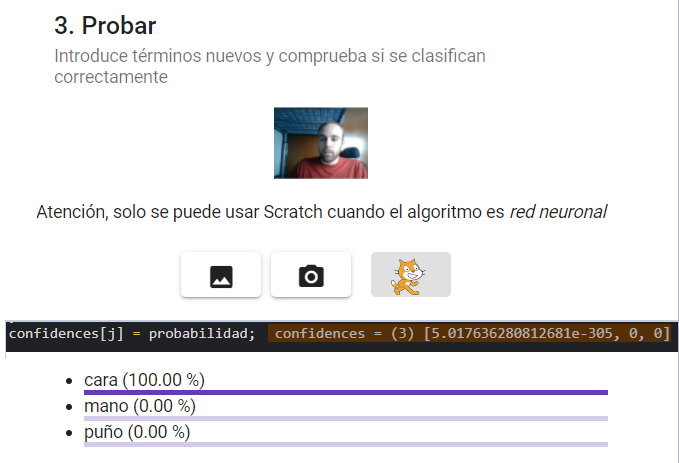
\includegraphics[width=9cm, keepaspectratio]{img/bayestestcara}
	\caption{Test de Bayes con los valores de las probabilidades obtenidas.}			
	\label{fig:bayestestcara}
\end{figure}

Se pueden hacer infinidad de operaciones matemáticas para intentar obtener unos valores algo más visibles aunque por supuesto, dependiendo de cuáles, ya \textbf{no} estaremos aplicando el algoritmo de Bayes como tal. Probando algunas, me di cuenta de que si hacemos sumatorio en vez de multiplicatorio estos números son algo más legibles. De nuevo con la misma entrada pero habiendo cambiado en el bucle la operación de multiplicación por una suma, obtenemos lo que vemos en la Figura~\ref{fig:bayestestcarasuma}.

\begin{figure}
	\centering
	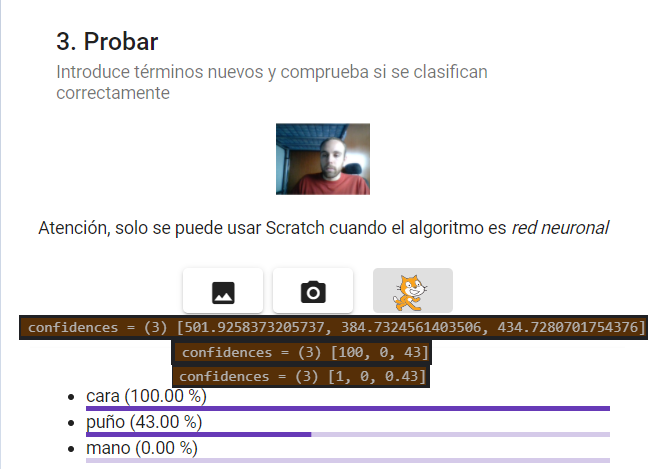
\includegraphics[width=9cm, keepaspectratio]{img/bayestestcarasuma}
	\caption{Test de Bayes de la etiqueta cara con los valores de las probabilidades obtenidas usando sumador en vez de multiplicador.}			
	\label{fig:bayestestcarasuma}
\end{figure}

En este caso, los números obtenidos son mucho más grandes, los podemos ver en los primeros valores de la variable \texttt{confidences}, aunque veamos números relativamente cercanos y que parecen del mimo orden, nos damos cuenta de que no es así ya que al normalizar, tanto entre 0 y 100 como entre 0 y 1, el segundo valor del array pasa a ser 0.

Probemos ahora a introducir la misma imagen de la etiqueta puño que usamos para el clasificador de K-NN. En la Figura~\ref{fig:bayestestpuno} podemos ver cómo en este caso también acierta aunque asigna un porcentaje bastante alto a la etiqueta cara. Aclarar que en Naive Bayes (aunque al estar haciendo sumatorio ya no sería Naive Bayes como tal, en el algoritmo original también puede ocurrir esto) los porcentajes de todas las etiquetas no tienen por qué sumar uno.

\begin{figure}
	\centering
	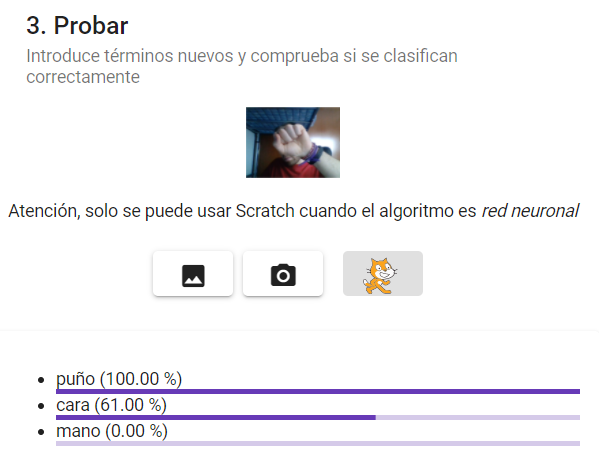
\includegraphics[width=9cm, keepaspectratio]{img/bayestestpuno}
	\caption{Test de Bayes de la etiqueta puño con los valores de las probabilidades obtenidas usando sumador en vez de multiplicador.}			
	\label{fig:bayestestpuno}
\end{figure}

En general este clasificador funciona bastante peor que los otros dos. Naive Bayes quizás funcione mejor para aplicaciones más simples o en las que no hay tantas características. Aún así si recordamos el ejemplo, vimos que los resultados para todas las etiquetas, incluso para la que más, eran bajos. Si con un ejemplo tan básico que solo tiene tres características y cada una de ellas pueden tomar dos y tres valores, en casos mucho más complejos con 1024 características y cinco valores para cada etiqueta, es normal que los valores sean ínfimos. Además, los vectores de características no sabemos de que es cada una, por tanto no podernos quedarnos solo con algunas o algo similar.
 
En definitiva, el algoritmo se ha implementado tal y cómo es y funciona correctamente, pero con ello nos hemos dado cuenta de que para utilizar Bayes tienen que ser casos más simples para que sea de utilidad.



%%%%%%%%%%%%%%%%%%%%%%%%%%%%%%%%%%%%%%%%%%%%%%%%%%%%%%%%%%%%%%%%%%%%%%%%%%%%%%%%
%%%%%%%%%%%%%%%%%%%%%%%%%%%%%%%%%%%%%%%%%%%%%%%%%%%%%%%%%%%%%%%%%%%%%%%%%%%%%%%%
% RESULTADOS %
%%%%%%%%%%%%%%%%%%%%%%%%%%%%%%%%%%%%%%%%%%%%%%%%%%%%%%%%%%%%%%%%%%%%%%%%%%%%%%%%

%\cleardoublepage
%\chapter{Resultados}

%En este capítulo se incluyen los resultados de tu trabajo fin de grado.

%Si es una herramienta de análisis lo que has realizado, aquí puedes poner ejemplos de haberla utilizado para que se vea su utilidad.


%%%%%%%%%%%%%%%%%%%%%%%%%%%%%%%%%%%%%%%%%%%%%%%%%%%%%%%%%%%%%%%%%%%%%%%%%%%%%%%%
%%%%%%%%%%%%%%%%%%%%%%%%%%%%%%%%%%%%%%%%%%%%%%%%%%%%%%%%%%%%%%%%%%%%%%%%%%%%%%%%
% CONCLUSIONES %
%%%%%%%%%%%%%%%%%%%%%%%%%%%%%%%%%%%%%%%%%%%%%%%%%%%%%%%%%%%%%%%%%%%%%%%%%%%%%%%%

\cleardoublepage
\chapter{Conclusiones}
\label{chap:conclusiones}

Creo que el resultado del trabajo ha sido bueno, teniendo en cuenta que quizás si hubiera tenido algo más de tiempo se podrían haber implementado algunas funciones más, las dos que más me llamaban la atención han quedado implementadas de manera correcta. De manera transversal a esto nos dimos cuenta de que teníamos que reestructurar la web y también se llevo a cabo.

\section{Consecución de objetivos}
\label{sec:consecucion-objetivos}

Si volvemos a los objetivos marcados para este proyecto, uno de los objetivos principales era reorganizar \texttt{LearningML}, esto se ha conseguido ya que se ha reestructurado la web en cuanto a componentes y servicios se refiere, ha quedado con una estructura mucho más limpia y fácil de mantener y ampliar para que en un futuro sea más sencillo implementar mejoras.

En cuanto al algoritmo de K-NN ha sido algo más fácil de implementar debido a que contábamos con la biblioteca de TensorFlow. Sin embargo, hubo que tratar los datos de entrada ya que por cómo se extraen las características no podíamos utilizarlos directamente, ya que en un primer lugar estaban pensados para el algoritmo de redes neuronales.

En el caso de Bayes estoy bastante orgulloso de haber conseguido implementarlo, me llevó bastantes mucho tiempo pasar el modelo en sí a lo que es lenguaje de programación, porque aunque entender el modelo no es tan difícil una vez lo tienes muy visto e interiorizado, hay que pensar cómo llevar eso a variables y funciones, además no me quedaba mucho tiempo para terminar y aunque el código es completamente funcional, seguro que se podría factorizar y optimizar. Aunque los resultados de este algoritmo no sean probabilidades coherentes, es así por cómo funciona, ya que al tener tantas características que pueden tomar tantos valores (incluso reduciéndolo a 5) las probabilidades para cada etiqueta son muy bajas, recordar de nuevo que estamos multiplicando 1024 números más pequeños que uno.


\section{Aplicación de lo aprendido}
\label{sec:aplicacion}

En la realización de este proyecto he puesto en práctica mis conocimientos adquiridos durante el grado sobre todo en cuestiones de modelos de aprendizaje, HTML, algo de CSS y JavaScript. Las demás asignaturas relacionadas con la programación también me han sido útiles de aunque se traten de lenguajes y tecnologías diferentes aportan conocimientos sobre el funcionamiento y la forma de desarrollar una aplicación.
 
Aunque no haya usado esos lenguajes como tal, todas las asignaturas de programación me han sido útiles, tanto Informática I como Informática II o Protocolos de transmisión de audio y vídeo. Lo mismo ocurre con Construcción de servicios y aplicaciones audiovisuales en internet o Laboratorio de tecnologías audiovisuales en la web donde se trabaja con JavaScript y algo de Node.js lo que me ha servido como base para utilizar TypeScript y el propio Node.js. Cabe destacar también que me llamó la atención implementar estos dos algoritmos de K-NN y Naive Bayes, porque ambos los habíamos visto en la asignatura de Tratamiento digital de la imagen y ya conocía su funcionamiento.

\section{Lecciones aprendidas}
\label{sec:lecciones_aprendidas}

Con las mejoras añadidas en la aplicación web \texttt{LearningML} he conseguido ampliar y mejorar los conocimientos adquiridos durante la carrera además de aprender otros totalmente nuevos. Entre ellos cabe destacar el aprendizaje de nuevas tecnologías que no había visto antes como por ejemplo:

\begin{enumerate}
  \item Angular: Aunque al principio tuve que dedicar bastante tiempo a entender cómo funcionaba, una vez lo comprendes todo te das cuenta de que facilita mucho el desarrollo y la programación. Es una herramienta muy potente que permite organizar una aplicación de cierto tamaño de manera más o menos sencilla, separando la parte del funcionamiento interno de la interfaz y a su vez permite pasar variables de una parte a otra. Es algo que si en un futuro intento crear una web de algún tipo lo tendré en cuenta.

  \item TypeScript: No me costó mucho adaptarme a este lenguaje y ahora que lo sé utilizar, diría que es más fácil entender cómo funciona un código en este lenguaje que en JavaScript.

  \item Programación asíncrona:  Aunque es un concepto que en sí no es complicado de entender, ya que consiste simplemente en que en ningún momento se bloquea el hilo principal y mientras se espera el resultado de algo el hilo principal continúa corriendo, a la hora de utilizarla es algo más complejo y tuve que pelearme bastante con ello hasta comprender su funcionamiento por completo y poder utilizarla.

  \item DevTools de Chrome: Aunque era una herramienta que ya conocía, no sabía la cantidad de cosas que te permite hacer, desde poner puntos de interrupción hasta imprimir cualquier variable en la consola. Esto es muy útil ya que puedes ir comprobando si el código esta funcionando como debería paso a paso.
\end{enumerate}



\section{Trabajos futuros}
\label{sec:trabajos_futuros}

Como ya se ha comentado en algún apartado anterior, las mejoras que se pueden añadir a la aplicación web \texttt{LearningML} son prácticamente infinitas. Vamos a ver algunas de ellas: 

\begin{itemize}
  	\item  Implementar nuevos tipos de datos de entrada como podría ser el sonido para así poder clasificar archivos de audio o grabaciones. Debido a la reestructuración que se ha llevado a cabo, "solo" habría que crear el archivo \texttt{feature-extractor-audio} y hacerlo de tal manera que las salidas tengan la misma estructura que ya tienen los otros dos archivos de extracción de características.

	\item Incluir otros modelos de aprendizaje como por ejemplo las máquinas de vectores de soporte.\footnote{\url{https://www.cienciadedatos.net/documentos/34_maquinas_de_vector_soporte_support_vector_machines}}

	\item Se podrían añadir como datos de entrada tablas de números directamente, que es algo muy interesante ya que hay modelos construidos en internet como por ejemplo el \emph{conjunto de datos iris}\footnote{\url{https://es.wikipedia.org/wiki/Conjunto_de_datos_flor_iris}} y se podrían cargar directamente o simplemente dejar que el usuario escriba a mano el valor numérico de las características que desee. 

	\item También queda por hacer la parte de relacionar los dos nuevos algoritmos implementados con Scratch, para poder crear el modelo desde ahí y después cargarlo en la propia web. 

	\item Otra idea podría ser modificar el diseño o añadir algún botón de información en el que se explique de manera sencilla como funciona cada algoritmo por dentro.
\end{itemize}


%%%%%%%%%%%%%%%%%%%%%%%%%%%%%%%%%%%%%%%%%%%%%%%%%%%%%%%%%%%%%%%%%%%%%%%%%%%%%%%%
%%%%%%%%%%%%%%%%%%%%%%%%%%%%%%%%%%%%%%%%%%%%%%%%%%%%%%%%%%%%%%%%%%%%%%%%%%%%%%%%
% APÉNDICE(S) %
%%%%%%%%%%%%%%%%%%%%%%%%%%%%%%%%%%%%%%%%%%%%%%%%%%%%%%%%%%%%%%%%%%%%%%%%%%%%%%%%

%\cleardoublepage
%\appendix
%\chapter{Manual de usuario}
%\label{app:manual}

%Esto es un apéndice.
%Si has creado una aplicación, siempre viene bien tener un manual de usuario.
%Pues ponlo aquí.

%%%%%%%%%%%%%%%%%%%%%%%%%%%%%%%%%%%%%%%%%%%%%%%%%%%%%%%%%%%%%%%%%%%%%%%%%%%%%%%%
%%%%%%%%%%%%%%%%%%%%%%%%%%%%%%%%%%%%%%%%%%%%%%%%%%%%%%%%%%%%%%%%%%%%%%%%%%%%%%%%
% BIBLIOGRAFIA %
%%%%%%%%%%%%%%%%%%%%%%%%%%%%%%%%%%%%%%%%%%%%%%%%%%%%%%%%%%%%%%%%%%%%%%%%%%%%%%%%

\cleardoublepage

% Las siguientes dos instrucciones es todo lo que necesitas
% para incluir las citas en la memoria
\bibliographystyle{abbrv}
\bibliography{memoria}  % memoria.bib es el nombre del fichero que contiene
% las referencias bibliográficas. Abre ese fichero y mira el formato que tiene,
% que se conoce como BibTeX. Hay muchos sitios que exportan referencias en
% formato BibTeX. Prueba a buscar en http://scholar.google.com por referencias
% y verás que lo puedes hacer de manera sencilla.
% Más información: 
% http://texblog.org/2014/04/22/using-google-scholar-to-download-bibtex-citations/

\end{document}
